\section{An example}\label{sec:Alg} 
As a demonstration of our method, we apply Theorem \ref{thm:trifunctor2} to prove that the bicategory of algebras, bimodules and bimodule homomorphisms in a bicategory ${\cat B}$ is monoidal and symmetric or braided, whenever this is true for ${\cat B}$. When ${\cat B}$ has only one object, more symmetry is preserved.
 As a result, the equivariant completion of a bicategory introduced in ~\cite{carquevillerunkel} preserves any symmetric, braided and monoidal structure, and the bicategory $CP({\bf C})$ of mixed quantum states introduced in ~\cite{heunenvicarywester} is symmetric monoidal.

\subsection{Overview}
Frobenius algebras and modules play an important role in quantum theory. Recently, the bicategory of Frobenius algebras, bimodules and bimodule homomorphisms has been defined independently in ~\cite{carquevillerunkel} and ~\cite{heunenvicarywester}, in different contexts. In ~\cite{carquevillerunkel} it is introduced as the equivariant completion of a bicategory, which is a tool for generating interesting topological quantum field theories. In ~\cite{heunenvicarywester} it has been introduced as the bicategory $2(CP({\bf C}))$ of mixed quantum states, which serves as the mathematical foundation for a diagrammatic language of quantum protocols. 

An essential question in either perspective is the existence of monoidal structures, which are braided or symmetric, for these categories. We will explore this question in generality for the bicategory $\mathcal{A}lg({\cat B})$, defined below.

\begin{defn}
Let ${\mathbb{D}}$ be a double category. We can define a new bicategory $\mathcal{A}lg({\mathbb{D}})$ consisting of the elements listed below.

\begin{itemize}
\item 0-cells are {\bf monoids} $(A,\tinymult[gray dot], \tinyunit[gray dot])$, in the monoidal category ${\mathbb{D}_1}$. Note that this requires that $S(A)=T(A)$.
\item 1-cells $(A,\tinymult[gray dot], \tinyunit[gray dot]) \mapsto (B,\tinymult[black dot], \tinyunit[black dot])$ are pairs (${\bf M}, M)$ of a $1-cell$ $M$ in $\doub{D}$ and a globular 2-cell ${\bf M}:A \times M \times B \rightarrow M$ in $\doub{D}$, with the structure of an $A-B-$bimodule. Note that $S(M) = T(A)$ and $T(M) = S(B)$. 
\item 2-cells are 2-morphisms $f:M \rightarrow N$ in ${\doub{D}}$ that are bimodule homomorphisms.
\end{itemize}

%\begin{itemize}
%\item 0-cells are {\bf monoids} $(A,\tinymult[gray dot], \tinyunit[gray dot])$, in the monoidal category ${\mathbb{D}_1}$. Note that this requires that $S(A)=T(A)$.
%\item 1-cells $(A,\tinymult[gray dot], \tinyunit[gray dot]) \mapsto (B,\tinymult[black dot], \tinyunit[black dot])$ are 1-cells ${\bf M}:A \rightarrow B$ with the structure of an $A-B-$bimodule.
%\item 2-cells are 2-morphisms in ${\cat B}$ that are bimodule homomorphisms.
%\end{itemize}
Structural data regarding this construction, such as horizontal composition, is described in ~\cite{carquevillerunkel}. 
\end{defn}


In \ref{sec:Dalg} we define the double category $\mathbb{A}lg({\mathbb{D}})$, whose horizontal bicategory corresponds to $\mathcal{A}lg({\doub{D}})$.  In \ref{sec:brmonDalg} and \ref{sec:fibDalg} we show that $\mathbb{A}lg({\doub{D}})$ is fibrant and that it is monoidal and braided or symmetric whenever this is true for ${\doub{D}}$. 
We will often refer to these categories as $\mathbb{A}lg$ and $\mathcal{A}lg$, when the choice of the original double category ${\doub{D}}$ is not important.


\subsection{Notation}
%Without loss of generality, we will assume that our bicategories are strict. We use the language of string diagrams for braided monoidal categories, first introduced by M. Kelly and M.L. Laplaza in ~\cite{kellylaplaza}, and its extended graphical calculus for monoidal bicategories described in ~\cite{bms}. In this diagrammatic language, we depict 0-cells as coloured surfaces, with the convention to use white for the unit 0-cell. We draw 1-cells (and identity 2-cells) as lines, and 2-cells generally as boxes between the source 1-cell in the bottom and the target 1-cell on top. We write horizontal composition $(\hor)$ and vertical composition $(\ver)$ in the horizontal and vertical direction, respectively. We write the tensor product $(\tens)$ as juxtaposition in the third direction, which is pointing into the paper. In our pictures this will be expressed as overlapping surfaces, as illustrated below. The reader who is not familiar with this graphical calculus may ignore the coloured surfaces and view the lines and boxes as string diagrams. This corresponds to the situation where the monoidal bicategory has only one object, which makes it a braided monoidal category. 
We use the language of string diagrams for braided monoidal double categories~\cite{bms}. In this diagrammatic language, we depict 0-cells as coloured surfaces, with the convention to use white for the unit 0-cell. We draw 1-cells (and identity 2-cells) as lines, and 2-cells generally as boxes between the source 1-cell in the bottom and the target 1-cell on top. We write loose composition $(\odot)$ and tight composition $(\circ)$ in the horizontal and vertical direction, respectively. We write the tensor product $(\tens)$ as juxtaposition in the third direction, which is pointing into the paper. In our pictures this will be expressed as overlapping surfaces, as illustrated below. The reader who is not familiar with this graphical calculus may ignore the coloured surfaces and view the lines and boxes as string diagrams. This corresponds to the situation where the monoidal bicategory has only one object, which makes it a braided monoidal category. 

\begin{equation*}
\mbox{[Update diagrams]}
\end{equation*}

\begin{align}
&\mbox{Loose composition} &\mbox{Tight composition} \hspace{28pt}
 &\mbox{Tensor product} \\
&
\begin{tikzpicture}[scale=1.75]
\draw[fill=red, draw=black, opacity=0.5] (-1,0) -- (-1,-2) -- (-.4,-2) -- (-.4,0) -- (-1,0);  
\draw[fill=blue, draw=black, opacity=0.5] (-.4,0) -- (-.4,-2) -- (.4,-2) -- (.4,0) -- (-.4,0); 
\draw[fill=green, draw=black, opacity=0.5] (.4,0) -- (.4,-2) -- (1,-2) -- (1,0) -- (.4,0);     
      \node[morphism, minimum width=10mm] (l) at (-.4,-1) {$f$};
      \draw (-.4,0) to (l.north);
      \draw (l.south) to (-.4,-2) node[below] {};
            \node[morphism, minimum width=10mm] (r) at (.4,-1) {$h$};
      \draw (.4,0) to (r.north);
      \draw (r.south) to (.4,-2) node[below] {};
    \end{tikzpicture}
 \hspace{10pt}
&       \begin{tikzpicture}[scale=1.75]
\draw[fill=red, draw=black, opacity=0.5] (-1,0) -- (-1,-2) -- (0,-2) -- (0,0) -- (-1,0);  
\draw[fill=blue, draw=black, opacity=0.5] (0,0) -- (0,-2) -- (1,-2) -- (1,0) -- (0,0);      
      \node[morphism, minimum width=10mm] (g) at (0,-.6) {$g$};
       \node[morphism, minimum width=10mm] (f) at (0,-1.4) {$f$};
       \draw (0,0) to (g.north);
      \draw (f.north) to (g.south);
      \draw (f.south) to (0,-2) node[below] {};
    \end{tikzpicture}
    \hspace{10pt}
&        \begin{tikzpicture}[scale=1.5]
\draw[fill=red, draw=black, opacity=0.5] (-1,0) -- (-1,-2) -- (0,-2) -- (0,0) -- (-1,0);  
\draw[fill=blue, draw=black, opacity=0.5] (0,0) -- (0,-2) -- (1,-2) -- (1,0) -- (0,0);      
      \node[morphism, minimum width=10mm] (l) at (0,-.8) {$f$};
      \draw (0,0) to (l.north);
      \draw (l.south) to (0,-2) node[below] {};
      %%%%%%%%%%%%%%%%%%%%%%%
      \draw[fill=purple, draw=black, opacity=0.5] (-.75,-.3) -- (-.75,-2.3) -- (0.25,-2.3) -- (0.25,-.3) -- (-.75,-.3);  
\draw[fill=green, draw=black, opacity=0.5] (0.25,-.3) -- (0.25,-2.3) -- (1.25,-2.3) -- (1.25,-.3) -- (0.25,-.3);      
      \node[morphism, minimum width=10mm] (l) at (0.25,-1.1) {$k$};
      \draw (0.25,-.3) to (l.north);
      \draw (l.south) to (0.25,-2.3) node[below] {};
    \end{tikzpicture}
\end{align}

\subsection{The double category $\Alg$}\label{sec:Dalg}
We will consider the abstract notion of a {\bf monoid} $(a,A, \tinymult[white dot], \tinyunit[white dot])$ in a double category {\doub{D}}. This is a 0-cell $a$ with a 1-cell $A$ such that $S(A)=T(A)=a$, a globular multiplication 2-cell $\tinymult[white dot]: A \odot A \rightarrow A$, and a globular unit 2-cell $\tinyunit[white dot]: U_a \rightarrow A$, that satisfy the associativity and unit law below. This makes $A$ a monoid in the usual sense in the monoidal category $\doub{D}_1$.

\begin{calign}
\label{eq:frobenius}
  \begin{pic}[yscale=0.85]
  \draw[fill=red, draw=black, opacity=.5] (-.9,-.5) -- (-.9,1) -- (1.4,1) -- (1.4,-.5) -- (-.9,-.5);
    \node[white dot] (l) at (0,0) {};
    \node[white dot] (r) at (.5,.5) {};
    \draw (l.center) to[out=90,in=180] (r.center);
    \draw (r.center) to (.5,1)node[above] {$A$};
    \draw (r.center) to[out=0,in=90] (1,-.5)node[below] {$A$};
    \draw (l.center) to[out=180,in=90] (-.5,-.5)node[below] {$A$};
    \draw (l.center) to[out=0,in=90] (.5,-.5)node [below] {$A$};
  \end{pic}
  \hspace{1pt}=\hspace{1pt}
  \begin{pic}[yscale=0.85]
\draw[fill=red, draw=black, opacity=.5] (-1.4,-.5) -- (-1.4,1) -- (.9,1) -- (.9,-.5) -- (-1.4,-.5);
    \node[white dot] (r) at (0,0) {};
    \node[white dot] (l) at (-.5,.5) {};
    \draw (r.center) to[in=0,out=90] (l);
    \draw (l.center) to (-.5,1)node[above] {$A$};
    \draw (l.center) to[in=90,out=180] (-1,-.5)node[below] {$A$};
    \draw (r.center) to[in=90,out=0] (.5,-.5)node[below] {$A$};
    \draw (r.center) to[in=90,out=180] (-.5,-.5)node[below] {$A$};
  \end{pic}
  \hspace{30pt}
  \begin{pic}[yscale=0.85]
  \draw[fill=red, draw=black, opacity=.5] (-.9,-.5) -- (-.9,1) -- (.9,1) -- (.9,-.5) -- (-.9,-.5);
    \node[white dot] (m) at (0,.5) {};
    \node[white dot] (u) at (-.5,0) {};
    \draw (m.center) to (0,1)node[above] {$A$};
    \draw (u.center) to[out=90,in=180] (m.center);
    \draw (m.center) to[out=0,in=90] (.5,-.5)node[below] {$A$};
  \end{pic}
  \hspace{1pt}=\hspace{1pt}
  \begin{pic}[yscale=0.85]
  \draw[fill=red, draw=black, opacity=.5] (-.9,-.5) -- (-.9,1) -- (.9,1) -- (.9,-.5) -- (-.9,-.5);
    \draw (0,-.5) node[below] {$A$} to (0,1) node[above]{$A$};
  \end{pic}
  \hspace{1pt}=\hspace{1pt}
  \begin{pic}[yscale=0.85]
    \draw[fill=red, draw=black, opacity=.5] (-.9,-.5) -- (-.9,1) -- (.9,1) -- (.9,-.5) -- (-.9,-.5);
    \node[white dot] (m) at (0,.5) {};
    \node[white dot] (u) at (.5,0) {};
    \draw (m.center) to (0,1)node[above] {$A$};
    \draw (u.center) to[out=90,in=0] (m.center);
    \draw (m.center) to[out=180,in=90] (-.5,-.5)node[below] {$A$};
  \end{pic}
\end{calign}

A {\bf monoid homomorphism} $(f, {\bf f}): (a, A, \tinymult[white dot], \tinyunit[white dot]) \rightarrow (b, B, \tinymult[gray dot], \tinyunit[gray dot])$ between two monoids is a 1-morphism $f:a\rightarrow b$ together with a 2-cell ${\bf f}:A \rightarrow B$ that respects the multiplication, $f \tinymult[white dot] = \tinymult[gray dot] (f odot f)$, and the unit, $\tinyunit[gray dot] = f \ver \tinyunit[white dot]$.
\begin{equation*}
\mbox{[insert picture]}
\end{equation*} 

If ${\doub{D}}$ is braided monoidal, then the {\bf category of monoids and monoid homomorphisms} is also braided monoidal. The tensor product for monoids in inherited from the original double category. This is depicted below. The unit object is the trivial monoid on the unit for the original monoidal structure with multiplication given by $\lambda_I = \rho_I$. The original structure isomorphisms are all monoid homomorphisms. In principle this can be shown directly, but in the diagrammatic calculus this holds trivially.  
\tikzset{region/.style={draw=black, fill opacity=0.75}}
\tikzset{regionA/.style={region, fill=red!50}}
\tikzset{regionB/.style={region, fill=blue!50}}
\begin{calign}
  \begin{pic}[xscale=3, yscale=2.25]
    \draw[regionA] (-1,-.4) -- (.4,-.4) -- (.4,1) -- (-1,1) -- (-1,-.4);
    \draw (-.5,0.5) to (-.5,1)node[above] {};
    \draw (.2,-.4) node[below]{} to[out=90,in=-90] (-.3,0);
    \draw (-.3,0) node[below]{} to[out=90,in=0] (-.5,0.5);
    \draw (-.5,0.5) to[out=180,in=90] (-.75,.1)node[below] {};
    \draw (-.75,.1) to[out=-90,in=90] (-.8,-.4)node[below] {};
    \node [white dot, node on layer=main] (m) at (-.5,.5) {};
    %%%%
    \draw[regionB] (-.9,-.5) -- (-.9,.9) -- (.5,.9) -- (.5,-.5) -- (-.9,-.5);
    \node[white dot] (m) at (0,.5) {};
    \draw (m.center) to (0,.9);
    \draw (.3,-.5) node[below]{} to[out=90,in=-90, looseness=1] (.25,.2);
    \draw (.25,.1) node[below]{} to[out=90,in=0, looseness=1] (m.center);
    \draw (m.center) to[out=180,in=0, looseness=1] (-.4,-.2)node[below] {};
    \draw (-.4,-.2) to[out=180,in=90, looseness=1] (-.7,-.5)node[below] {};
  \end{pic}
\end{calign}



An A,B-{\bf bimodule} $(M, {\bf M})$ in {\doub{D}} is 1-cell $M: a \hto b$, together with a globular 2-cell ${\bf M}: A \odot M \odot  B \rightarrow M$, satisfying the composition and unit law below.

\begin{equation*}
\mbox{[Add region labels and colors}]
\end{equation*}
\begin{equation}\label{eq:bimodule}
    \begin{pic}[yscale=0.85]
      \node[morphism, minimum width=10mm] (u) at (0,0) {$\mathbf{M}$};
      \node[morphism, minimum width=10mm] (l) at (0,-1.1) {$\mathbf{M}$};
      \draw (u.north) to (0,.6) node[right] {$M$};
      \draw (u.south) to (l.north);
      \draw (l.south) to (0,-2) node[right] {$M$};
      \draw (l.-45) to[out=-90,in=90] (.6,-2) node[right] {$B$};
      \draw (l.-135) to[out=-90,in=90] (-.6,-2) node[right] {$A$};
      \draw (u.-45) to[out=-90,in=90] (1.1,-1) to (1.1,-2) node[right] {$B$};
      \draw (u.-135) to[out=-90,in=90] (-1.1,-1) to (-1.1,-2) node[right] {$A$};
    \end{pic}
    =
    \begin{pic}[yscale=0.85]
      \node[morphism, minimum width=10mm] (m) at (0,0) {$\mathbf{M}$};
      \node[white dot] (l) at (-.85,-1) {};
      \node[black dot] (r) at (.85,-1) {};
      \draw (m.north) to (0,.6) node[right] {$M$};
      \draw (m.south) to (0,-2) node[right, xshift=-.2] {$M$};
      \draw (m.-45) to[out=-90,in=90] (r);
      \draw (m.-135) to[out=-90,in=90] (l);
      \draw (l) to[out=-150,in=90] (-1.1,-2) node[left] {$A$};
      \draw (l) to[out=-30,in=90] (-.6,-2) node[left] {$A$};
      \draw (r) to[out=-150,in=90] (.6,-2) node[right] {$B$};
      \draw (r) to[out=-30,in=90] (1.1,-2) node[right] {$B$};
    \end{pic}
    \qquad
    \begin{pic}[yscale=0.85]
      \draw (0,.6) node[right] {$M$} to (0,-2) node[right] {$M$};
    \end{pic}
    \!\!\!=\,\,\,
    \begin{pic}[yscale=0.85]
      \node[morphism, minimum width=10mm] (m) at (0,0) {$\mathbf{M}$};
      \draw (m.north) to (0,.6) node[right] {$M$};
      \draw (m.south) to (0,-2) node[right] {$M$};
      \draw (m.-135) to[out=-90,in=90] +(0,-0.75) node[white dot] {};
      \draw (m.-45) to[out=-90,in=90] +(0,-0.75) node[black dot] {};
    \end{pic}
  \end{equation}
For readability, we sometimes write A-B-bimodules ${\bf M}$ as $_A{\bf M}_B$ and we abbreviate the following compositions: ${}_{\tinydot[white dot]}{\bf M} := {\bf M} (\tinyunit[white dot] \tens \mathid)$, ${\bf M}_{\tinydot[gray dot]}:= {\bf M}  (\mathid \tens \tinyunit[gray dot])$, and $_{\tinydot[white dot]}{\bf M}_{\tinydot[gray dot]}:= {\bf M}  (\tinyunit[white dot] \tens \tinyunit[gray dot])$. An {\bf extended bimodule homomorphism} ${\bf f}: {\bf M} \rightarrow {\bf N}$ is a triple of 2-cells $(A \xrightarrow{\bf f_l} C, M \xrightarrow{\bf f} N, B \xrightarrow{\bf f_r} D)$ in $\doub{D}$ such that $f  {\bf M} = {\bf N}  (f_l \odot f \odot f_r)$.
\begin{equation*}
\mbox[insert picture]
\end{equation*}
 When ${\bf f_l}$ and ${\bf f_r}$ are identities and {\bf f} is globular, this corresponds to the standard definition of a {\bf bimodule homomorphism}.
Bimodules and extended bimodule homomorphisms in a monoidal double category {\doub{D}} form a braided monoidal category, where the tensor product on objects is inherited from {\doub{B}}, see the picture below. On morphisms, it is defined as $({\bf f_l},{\bf f},{\bf  f_r})\tens ({\bf g_l}, {\bf g}, {\bf g_r}) = ({\bf f_l} \tens {\bf g_l}, {\bf f} \tens {\bf g}, {\bf f_r} \tens {\bf g_r})$. The unit object corresponds to the bimodule given by the coherence map depicted below. 

\begin{equation}
{\bf I}:= \quad
\smash{{\hspace{-5pt}\ensuremath{\begin{pic}[scale=1.5,string,yscale=-1.5]
\draw (-1,0) -- (1,0) -- (1,1) -- (-1,1) -- (-1,0);
      \node (0) at (0,0) {};
      \node[gray dot, inner sep=1.5pt] (1) at (0,0.55) {};
      \node (2) at (-0.5,1) {};
      \node (3) at (0.5,1) {};
      \draw (0.center)node[above]{$U_I$} to (1.center);
      \draw (1.center) to [out=left, in=down, out looseness=1.5] (2.center)node[below]{$U_I$};
      \draw (1.center) to [out=right, in=down, out looseness=1.5] (3.center)node[below]{$U_I$};
      \draw (1.center) to (0,1)node[below]{$U_I$};
      \end{pic}}\hspace{-3pt}}}
\hspace{30pt}
\tikzset{region/.style={draw=black, fill opacity=0.75}}
\tikzset{regionA/.style={region, fill=red!50}}
\tikzset{regionB/.style={region, fill=blue!50}}
\tikzset{regionC/.style={region, fill=purple!50}}
\tikzset{regionD/.style={region, fill=green!50}}
_A{\bf M}_B \tens {}_C{\bf N}_D :=
   \ensuremath{\begin{pic}[scale=1.5]
\draw[regionA] (-1,0) -- (-1,-2) -- (0,-2) -- (0,0) -- (-1,0);  
\draw[regionB] (0,0) -- (0,-2) -- (2,-2) -- (2,0) -- (0,0);      
      \node[morphism, minimum width=10mm] (l) at (0,-.8) {$\mathbf{M}$};
      \draw (0,0) to (l.north);
      \draw (l.south) to (0,-2) node[below] {};
      \draw (l.-45) to[out=-90,in=90] (1.5,-2) node[below] {};
      \draw (l.-135) to[out=-90,in=90] (-.6,-2) node[below] {};
      %%%%%%%%%%%%%%%%%%%%%%%
      \draw[regionC] (-.9,-.1) -- (-.9,-2.1) -- (1.1,-2.1) -- (1.1,-.1) -- (-.9,-.1);  
\draw[regionD] (1.1,-.1) -- (1.1,-2.1) -- (2.1,-2.1) -- (2.1,-.1) -- (1.1,-.1);      
      \node[morphism, minimum width=10mm] (l) at (1.1,-.8) {$\mathbf{N}$};
      \draw (1.1,-.1) to (l.north);
      \draw (l.south) to (1.1,-2.1) node[below] {};
      \draw (l.-45) to[out=-90,in=90] (1.7,-2.1) node[below] {};
      \draw (l.-135) to[out=-90,in=90] (-.4,-2.1) node[below] {};
    \end{pic}}
\end{equation}

\begin{equation*}
\mbox{[Add region labels 'I']}
\end{equation*}

The associator, unitor, and swap natural isomorphisms are given by the maps with the following components, where $\alpha, \lambda$, and $\rho$ are the structure isomorphisms of the original monoidal double category. 

\begin{align}
 {\bf \alpha}_{_A{\bf M}_B,_C{\bf N}_D,_E{\bf P}_F} &:= ({\bf \alpha}_{A,C,E}, {\bf \alpha}_{M,N,P}, {\bf \alpha}_{B,D,F}) 
\\{\bf \lambda}_{_A{\bf M}_B}&:= ({\bf \lambda}_A, {\bf \lambda}_M, {\bf \lambda}_B)
\\{\bf \rho}_{_A{\bf M}_B} &:= ({\bf \rho}_A, {\bf \rho}_M, {\bf \rho}_B)
\\{\bf \sigma}_{\bf {}_AM_B,{}_CN_D}&: = ({\bf \sigma}_{A,C}, {\bf \sigma}_{M,N}, {\bf \sigma}_{B,D})
\end{align}

For clarity we write monoids and monoid homomorphisms in normal font and we write bimodules and (extended) bimodule homomorphisms in bold. This will help distinguishing between the two categories, which together form a double category.

\begin{lem}\label{lem:algdouble}
Let ${\doub{D}}$ be a double category such that all coequalizers exist in $\doub{D}_1$, and where horizontal composition $\odot$ preserves coequalizers. The category of monoids and monoid homomorphisms of ${\doub{D}}$ and the category of bimodules and extended bimodule homomorphisms of ${\doub{D}}$ together form a double category, which we call $\Alg[\doub{D}]$
\end{lem}

\begin{proof}
The {\bf unit functor} $\Alg[\doub{D}]_0 \xrightarrow{U} \Alg[\doub{D}]_1$ is defined on objects as $U(a,A,\tinymult[gray dot],\tinyunit[gray dot]) := 
     (A, \smash{{\hspace{-5pt}\ensuremath{\begin{pic}[scale=0.4,string,yscale=-1]
      \node (0) at (0,0) {};
      \node[gray dot, inner sep=1.5pt] (1) at (0,0.55) {};
      \node (2) at (-0.5,1) {};
      \node (3) at (0.5,1) {};
      \draw (0.center) to (1.center);
      \draw (1.center) to [out=left, in=down, out looseness=1.5] (2.center);
      \draw (1.center) to [out=right, in=down, out looseness=1.5] (3.center);
      \draw (1.center) to (0,1);
      \end{pic}}\hspace{-3pt}}})$; 
      and on morphisms as $U({\bf f}) := ({\bf f},{\bf f},{\bf f})$. The {\bf source and target functors} $S,T: \lD_1 \rightarrow \lD_0$ are defined on objects as $S({}_A {\bf M}_B) = A$, and  $T({}_A {\bf M}_B) = B$, and on morphisms as  $S({\bf f_l},{\bf f},{\bf f_r})={\bf f_l}$, and $T({\bf f_l}, {\bf f}, {\bf f_r}) = {\bf f_r}$.
The functor ${\Alg[\doub{D}]_1} \times_{\Alg[\doub{D}]_0} {\Alg[\doub{D}]_1} \rightarrow {\Alg[\doub{D}]_1}$, maps objects $(_A{\bf M}_B$, $_B{\bf N}_C)$ to $_A{\bf M} \tinydot[gray dot] {\bf N}_C$, and morphisms $(({\bf f_l}, {\bf f}, {\bf h}), ({\bf h}, {\bf g}, {\bf g_r}))$ to $({\bf f_l}, {\bf f \tinydot[gray dot] g}, {\bf g_r})$, where ${M} \tinydot[gray dot] {N}$ and $f \tinydot[gray dot] g$ are defined by the following coequalisers:

\begin{equation}\label{eq:coequaliser}
  \begin{pic}[xscale=4,yscale=1.66, thin]
    \node (tl) at (-.3,1) {$M \odot B \odot N$};
    \node (bl) at (-.3,0) {$M' \odot B' \odot N'$};
    \node (t) at (1,1) {$M \odot N$};
    \node (b) at (1,0) {$M' \odot N'$};
    \node (tr) at (1.7,1) {$M \tinydot[gray dot] N$};
    \node (br) at (1.7,0) {$M' \tinydot[gray dot] N'$};
    \draw[->] (tl) to node[left] {$({\bf f} \odot {\bf h} \odot {\bf g})$} (bl);
    \draw[->] (t) to node[right] {${\bf f} \odot {\bf g}$} (b);
    \draw[->, dashed] (tr) to node[right] {${\bf f} \tinydot[gray dot] {\bf g}$} (br);
    \draw[->] (t) to node[above] {$c$} (tr);
    \draw[->] (b) to node[below] {$c'$} (br);
    \draw[->] ([yshift=1.5pt]tl.east) to node[above] {${}_{\tinydot[white dot]}\mathbf{M} \odot \mathid_{N}$} ([yshift=1.5pt]t.west);
    \draw[->] ([yshift=-1.5pt]tl.east) to node[below] {$\mathid_{M} \odot \mathbf{N}_{\tinydot[black dot]}$} ([yshift=-1.5pt]t.west);
    \draw[->] ([yshift=1.5pt]bl.east) to node[above] {${}_{\tinydot[white dot]}\mathbf{M'} \odot \mathid_{N'}$} ([yshift=1.5pt]b.west);
    \draw[->] ([yshift=-1.5pt]bl.east) to node[below] {$\mathid_{M'} \odot \mathbf{N'}_{\tinydot[black dot]}$} ([yshift=-1.5pt]b.west);
  \end{pic}
 \end{equation}

By commutativity of the left square, $c ({\bf f} \odot {\bf g})$ is another coequaliser of the upper two parallel maps, hence $f \tinydot[gray dot] g$ exists and is unique. 
  The module ${\bf M} \tinydot[gray dot] {\bf N}$ is given by the map that makes the diagram below commute. It exists and is unique by uniqueness of coequalisers, taking commutativity of the left square into account, and the fact that horizontal composition preserves coequalisers. 

\begin{equation}\label{eq:coequaliser2}
  \begin{pic}[xscale=4,yscale=1.66, thin]
    \node (tl) at (-.3,1) {$A \odot M \odot B \odot N \odot C$};
    \node (bl) at (-.3,0) {$M \odot B \odot N$};
    \node (t) at (1,1) {$A \odot M \odot N \odot C$};
    \node (b) at (1,0) {$M \odot N$};
    \node (tr) at (1.7,1) {$A \odot M \tinydot[gray dot] N \odot C$};
    \node (br) at (1.7,0) {$M \tinydot[gray dot] N$};
    \draw[->] (tl) to node[left] {${\bf M}_{\tinydot[gray dot]} \odot \mathid_B \odot {}_{\tinydot[gray dot]}{\bf N}$} (bl);
    \draw[->] (t) to node[right] {${\bf M}_{\tinydot[gray dot]} \odot  {}_{\tinydot[gray dot]}{\bf N}$} (b);
    \draw[->, dashed] (tr) to node[right] {${\bf M} \tinydot[gray dot] {\bf N}$} (br);
    \draw[->] (t) to node[above] {$\mathid_A \odot c \odot \mathid_C$} (tr);
    \draw[->] (b) to node[below] {$c$} (br);
    \draw[->] ([yshift=1.5pt]tl.east) to node[above] {$\mathid_A \odot {}_{\tinydot[white dot]}\mathbf{M} \odot \mathid_N \odot \mathid_C$} ([yshift=1.5pt]t.west);
    \draw[->] ([yshift=-1.5pt]tl.east) to node[below] {$\mathid_A \odot \mathid_M \odot \mathbf{N}_{\tinydot[black dot]} \odot \mathid_C$} ([yshift=-1.5pt]t.west);
    \draw[->] ([yshift=1.5pt]bl.east) to node[above] {${}_{\tinydot[white dot]}\mathbf{M'} \odot \mathid_{N'}$} ([yshift=1.5pt]b.west);
    \draw[->] ([yshift=-1.5pt]bl.east) to node[below] {$\mathid_{M'} \odot \mathbf{N'}_{\tinydot[black dot]}$} ([yshift=-1.5pt]b.west);
  \end{pic}  
 \end{equation}

Note that ${\bf N}_{\tinydot[gray dot]} \odot {}_{\tinydot[gray dot]}{\bf N}$ is a module. It is easy to check that ${\bf M}_{\tinydot[gray dot]}{\bf N}$ satisfies the module axioms as well, using commutativity of the diagram above and the fact that $c$ is epic. Pasting the two diagrams together into a cube proves that ${\bf f} \odot {\bf g}$ is a bimodule homomorphism.
 
It is left to verify functoriality of ${\Alg[\doub{D}]_1} \times_{\Alg[\doub{D}]_0} {\Alg[\doub{D}]_1} \rightarrow {\Alg[\doub{D}]_1}$. When we unfold the definitions we see that we only need to check that $({\bf f}\tinydot[gray dot]{\bf f'}) \circ ( {\bf g} \tinydot[gray dot] {\bf g'}) = ({\bf f} \circ {\bf f'})\tinydot[gray dot] ({\bf g} \circ {\bf g'})$, and $\mathid_{\bf M} \tinydot[gray dot] \mathid_{\bf M'} = \mathid_{\bf M \tinydot[gray dot] M'}$. The two sides of the first equality are the unique maps making the two diagram below commute. If we forget the middle part of the left diagram, the diagrams are equal by the exchange law for $\odot$ and $\circ$. As a consequence, the dashed arrows of the two diagrams must be equal too. A similar argument shows that $\mathid_{\bf M} \tinydot[gray dot] \mathid_{\bf M'} = \mathid_{\bf M \tinydot[gray dot] M'}$.
 
 \begin{equation}
  \begin{pic}[xscale=2.3, yscale=1.5, thin]
    \node (tl) at (-.3,1) {$M \hor B \hor N$};
    \node (bl) at (-.3,0) {$L \hor C \hor K$};
    \node (ld) at (-.3,-1) {$P \hor D \hor Q$};
    \node (t) at (1,1) {$M \hor N$};
    \node (b) at (1,0) {$L \hor K$};
    \node (md) at (1,-1) {$P \hor Q$};
    \node (tr) at (1.7,1) {${M}_{\tinydot[gray dot]} {N}$};
    \node (br) at (1.7,0) {${K}_{\tinydot[gray dot]} {L}$};
    \node (rd) at (1.7,-1) {${M}_{\tinydot[gray dot]} {N}$};
    \draw (tl) to  (-.3,.65);
    \node at (-.3, 0.5) {$f \hor i \hor g$};
    \draw[->] (-.3,.35) to  (bl);
    \draw[->] (t) to node[right] {$f \hor g$} (b);
    \draw[->, dashed] (tr) to node[right] {$f_{\tinydot[gray dot]}g$} (br);
    \draw[->, dashed] (br) to node[right] {$h_{\tinydot[gray dot]}k$} (rd);
    \draw[->] (t) to node[above] {$c_B$} (tr);
    \draw[->] (b) to node[below] {$c_C$} (br);
    \draw[->] ([yshift=1.5pt]tl.east) to node[above] {${}_{\tinydot[white dot]}\mathbf{M} \hor \mathid_{N}$} ([yshift=1.5pt]t.west);
    \draw[->] ([yshift=-1.5pt]tl.east) to node[below] {$\mathid_{M} \hor \mathbf{N}_{\tinydot[black dot]}$} ([yshift=-1.5pt]t.west);
    \draw[->] ([yshift=1.5pt]bl.east) to node[above] {${}_{\tinydot[white dot]}\mathbf{K} \hor \mathid_{L}$} ([yshift=1.5pt]b.west);
    \draw[->] ([yshift=-1.5pt]bl.east) to node[below] {$\mathid_{K} \hor \mathbf{L}_{\tinydot[black dot]}$} ([yshift=-1.5pt]b.west);
    \draw (bl) to  (-.3,-.35);
    \node at (-.3,-.5) {$h \hor j \hor k$};
    \draw[->] (-.3,-.65) to  (ld);
    \draw[->] (b) to node[right] {$h \hor k$} (md);
   % \draw[->, dashed] (tr) to node[right] {$\rho_M \tinydot[gray dot] \rho_N$} (rd);
    \draw[->] (md) to node[above] {$c_D$} (rd);
    \draw[->] ([yshift=1.5pt]ld.east) to node[above] {${}_{\tinydot[white dot]}\mathbf{P} \hor \mathid_{Q}$} ([yshift=1.5pt]md.west);
    \draw[->] ([yshift=-1.5pt]ld.east) to node[below] {$\mathid_{P}  \hor \mathbf{Q}_{\tinydot[black dot]}$} ([yshift=-1.5pt]md.west);
%    \draw[->, dashed] (br) to [in=90, out=90] {$\hat{\xi}^{-1}$} (rd);
  \end{pic}  
   \begin{pic}[xscale=2.3, yscale=1.5, thin]
    \node (tl) at (-.3,1) {$M \hor B \hor N$};
    \node (ld) at (-.3,-1) {$P \hor D \hor Q$};
    \node (t) at (1,1) {$M \hor N$};
    \node (md) at (1,-1) {$P \hor Q$};
    \node (tr) at (1.7,1) {${M}_{\tinydot[gray dot]} {N}$};
    \node (rd) at (1.7,-1) {${M}_{\tinydot[gray dot]} {N}$};
    \draw (tl) to  (-.3,0.25);
    \draw[->] (-.3,-0.25) to  (ld);
    \node at (-.3,0.125) {$(k \ver f) \hor (j \ver i)$};
    \node at (-.3,-.125) {$\hor (k \ver g)$};
    \draw (t) to  (1,0.3);
    \draw[->] (1,0.1) to  (md);
    \node at (1,0.2) {$(h \ver f) \hor (k \ver g)$};
    \draw[dashed] (tr) to (1.7,-0.1);
    \node at (1.7,-.2) {$(h \ver f)_{\tinydot[gray dot]}(k \ver g)$};
    \draw[->, dashed] (1.7,-0.3) to (rd); 
    \draw[->] (t) to node[above] {$c_B$} (tr);
    \draw[->] ([yshift=1.5pt]tl.east) to node[above] {${}_{\tinydot[white dot]}\mathbf{M} \hor \mathid_{N}$} ([yshift=1.5pt]t.west);
    \draw[->] ([yshift=-1.5pt]tl.east) to node[below] {$\mathid_{M} \hor \mathbf{N}_{\tinydot[black dot]}$} ([yshift=-1.5pt]t.west);
    \draw[->] (md) to node[above] {$c_D$} (rd);
    \draw[->] ([yshift=1.5pt]ld.east) to node[above] {${}_{\tinydot[white dot]}\mathbf{P} \hor \mathid_{Q}$} ([yshift=1.5pt]md.west);
    \draw[->] ([yshift=-1.5pt]ld.east) to node[below] {$\mathid_{P}  \hor \mathbf{Q}_{\tinydot[black dot]}$} ([yshift=-1.5pt]md.west);
  \end{pic}
 \end{equation}

The {\bf associator} ${\bf a}: ({\bf M_1} \ominus {\bf M_2}) \ominus {\bf M_3} \rightarrow {\bf M_1} \ominus ({\bf M_2} \ominus {\bf M_3})$ is an the extended algebra homomorphism of the form $(\mathid, a, \mathid)$. Let $\pi_1$ and $\pi_2$ be two different coequalisers of the maps depicted below. Then $a_{M_1,M_2,M_3}$ is defined as the unique isomorphism between their images.
Similarly we derive the component $a_{N_1,N_2,N_3}$. Naturality of $a$ follows from the rightmost square of the diagram, which commutes because all other sub diagrams commute. 

\begin{tikzpicture}[xscale=5,yscale=2.5]
 \node (tl) at (0,1) {$M_1 \hor B \hor M_2 \hor C \hor M_3$};
 \node (bl) at (0,0) {$N_1 \hor D \hor N_2 \hor E \hor N_3$};
  \node (tm) at (1,1) {$M_1 \hor M_2 \hor M_3$};
 \node (bm) at (1,0) {$N_1 \hor N_2 \hor N_3$};
\draw[->] ([yshift=1.5pt] tl.east) to node[above] {$_{\tinydot [gray dot]}{\bf M_1} \hor {}_{\tinydot[gray dot]}{\bf M_2} \hor \mathid_{M_3}$} ([yshift=1.5pt] tm.west);
\draw[->] ([yshift=-1.5pt] tl.east) to node[below] {$\mathid_{M_1} \hor {\bf M_2}_{\tinydot[gray dot]} \hor  {\bf M_3}_{\tinydot[gray dot]}$} ([yshift=-1.5pt] tm.west);
\draw[->] ([yshift=1.5pt] bl.east) to node[above] {$_{\tinydot [gray dot]}{\bf N_1} \hor {}_{\tinydot[gray dot]}{\bf N_2} \hor \mathid_{N_3}$} ([yshift=1.5pt] bm.west);
\draw[->] ([yshift=-1.5pt] bl.east) to node[below] {$\mathid_{N_1} \hor {\bf N_2}_{\tinydot[gray dot]} \hor  {\bf N_3}_{\tinydot[gray dot]}$} ([yshift=-1.5pt] bm.west);
 \node (r1) at (2,1.25) {$({M_1}_{\tinydot[gray dot]} {M_2})_{\tinydot[gray dot]} {M_3}$};
 \node (r2) at (1.6,0.75) {${M_1}_{\tinydot[gray dot]} ({M_2}_{\tinydot[gray dot]} M_3)$};
  \node (r3) at (2,0.25) {$({N_1}_{\tinydot[gray dot]} {N_2})_{\tinydot[gray dot]} N_3$};
 \node (r4) at (1.6,-0.25) {${N_1}_{\tinydot[gray dot]} ({N_2}_{\tinydot[gray dot]} N_3)$};
 \draw[->] (tm) to node[above] {$\pi_1$} (r1.west);
 \draw[->] (tm) to node[below] {$\pi_2$} (r2);
  \draw[->] (bm) to node[above] {$\phi_1$} (r3.west);
 \draw[->] (bm) to node[below] {$\phi_2$} (r4);
  \draw[->, dashed] (r1) to node[left] {$a_{M_1,M_2,M_3}$} (r2);
 \draw[->, dashed] (r3) to node[right] {$a_{N_1,N_2,N_3}$} (r4);
  \draw[->, dashed] (r1) to node[right] {$(f_1 \tinydot[gray dot] f_2) \tinydot[gray dot] f_3$} (r3);
 \draw[->, dashed, cross] (r2) to node[left, yshift=14pt] {$f_1 \tinydot[gray dot] (f_2 \tinydot[gray dot] f_3)$} (r4);
 \draw (tl) to (0,0.6) node[below]{$f_1 \hor f_B \hor f_2 \hor f_C \hor f_3$};
  \draw[->] (0,0.4) to (bl);
 \draw[->] (tm) to node[left] {$f_1 \hor f_2 \hor f_3$} (bm); 
\end{tikzpicture}

The coequalisers $\pi_1$ and $\pi_2$ correspond to the compositions of coequalisers below. 

\begin{equation}
\pi_1 :=
\begin{aligned}
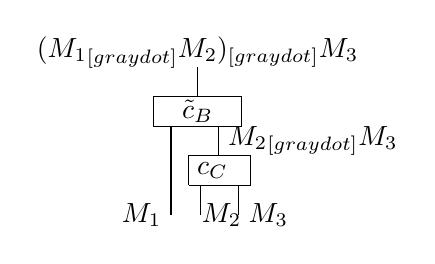
\begin{tikzpicture}[scale=0.75]
\node at (0.75,1.25) {$({M_1}_{\tinydot[gray dot]} {M_2})_{\tinydot[gray dot]} {M_3}$};
\draw (0,0) -- (0,0.5) -- (1.5, 0.5) -- (1.5,0) -- (0,0);
\node at (0.75,0.25) [] {$\tilde{c}_B$};
\draw (0.75,0.5) to  (0.75,1);
\draw (0.3,0) -- (0.3,-1.5)node[left]{$M_1$};
\draw  (1.1,0) to node[right]{${M_2}_{\tinydot[gray dot]}M_3$} (1.1,-0.5);
\draw (0.6,-1) -- (0.6,-0.5) -- (1.65, -0.5) -- (1.65,-1) -- (0.6,-1);
\node at (1,-0.75) [] {$c_C$};
\draw (0.8,-1) to (0.8,-1.5)node[right,xshift=-3pt]{$M_2$}; 
\draw (1.45,-1) -- (1.45,-1.5)node[right]{$M_3$};
\end{tikzpicture}
\end{aligned}
\hspace{.5cm}
\pi_2:=
\begin{aligned}
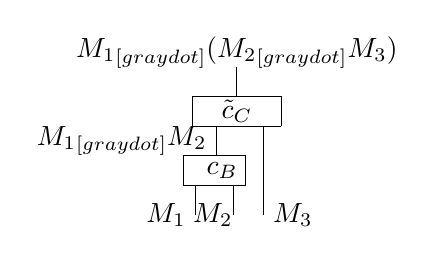
\begin{tikzpicture}[xscale=-0.75, yscale=0.75]
\node at (0.75,1.25) {${M_1}_{\tinydot[gray dot]} ({M_2}_{\tinydot[gray dot]} {M_3})$};
\draw (0,0) -- (0,0.5) -- (1.5, 0.5) -- (1.5,0) -- (0,0);
\node at (0.75,0.25) [] {$\tilde{c}_C$};
\draw (0.75,0.5) -- (0.75,1);
\draw (0.3,0) -- (0.3,-1.5)node [right]{$M_3$};
\draw  (1.1,0) to node[left]{${M_1}_{\tinydot[gray dot]}M_2$} (1.1,-0.5);
\draw (0.6,-1) -- (0.6,-0.5) -- (1.65, -0.5) -- (1.65,-1) -- (0.6,-1);
\node at (1,-0.75) [] {$c_B$};
\draw (0.8,-1) to (0.8,-1.5)node [left,xshift=3pt]{$M_2$}; 
\draw (1.45,-1) to (1.45,-1.5)node[left]{$M_1$};
\end{tikzpicture}
\end{aligned}
\end{equation}

The equations below express the fact that $\pi_1$ is a cocone of $_{\tinydot [gray dot]}{\bf M_1} \hor {}_{\tinydot[gray dot]}{\bf M_2} \hor \mathid_{M_3}$ and $\mathid_{M_1} \hor {\bf M_2}_{\tinydot[gray dot]} \hor  {\bf M_3}_{\tinydot[gray dot]}$.

\begin{equation}
\begin{aligned}
\begin{tikzpicture}[xscale=0.8,yscale=0.7]
\node at (0.75,1.25) {$({M_1}_{\tinydot[gray dot]} {M_2})_{\tinydot[gray dot]} {M_3}$};
\draw (0,0) -- (0,0.5) -- (1.5, 0.5) -- (1.5,0) -- (0,0);
\node at (0.75,0.25) [] {$\tilde{c}_B$};
\draw (0.75,0.5) -- (0.75,1);
\draw (0.3,0) to[in=90,out=-90] (-0.1,-1.5);
\draw  (1.1,0) -- (1.1,-0.5);
\draw (0.6,-1) -- (0.6,-0.5) -- (1.65, -0.5) -- (1.65,-1) -- (0.6,-1);
\node at (1.1,-0.75) [] {$c_C$};
\draw (0.8,-1) to (0.8,-1.5); 
\draw (1.45,-1) to[in=90,out=-90] (1.85,-3);
\draw (-0.5,-2) -- (0.3, -2) -- (0.3, -1.5) -- (-0.5,-1.5) -- (-0.5,-2);
\node at (-0.1, -1.75) {$\bf M_1$};
\draw (0.4,-2) -- (1.2,-2) -- (1.2,-1.5) -- (0.4,-1.5) -- (0.4,-2);
\draw (-0.4,-2) to (-0.4,-2.25) node[gray dot]{};
\draw (-0.1,-2) -- (-0.1,-3);
\draw (0.2,-2) -- (0.2,-3);
\draw (0.5,-2) to (0.5,-2.25) node[gray dot]{};
\draw (0.8,-2) to (0.8,-3);
\draw (1.1,-2) to[in=90,out=-90] (1.3,-3);
\node at (0.8,-1.75) {$\bf M_2$};
\node at (-0.1,-3.25) [] {$M_1$};
\node at (0.3,-3.25) [] {$B$};
\node at (0.8,-3.25) [] {$M_2$};
\node at (1.3,-3.25) [] {$C$};
\node at (1.85,-3.25) [] {$M_3$};
\end{tikzpicture}
\end{aligned}
=
\begin{aligned}
\begin{tikzpicture}[xscale=1.2,yscale=0.7]
\node at (0.75,1.25) {$({M_1}_{\tinydot[gray dot]} {M_2})_{\tinydot[gray dot]} {M_3}$};
\draw (0,0) -- (0,0.5) -- (1.5, 0.5) -- (1.5,0) -- (0,0);
\node at (0.75,0.25) [] {$\tilde{c}_B$};
\draw (0.75,0.5) -- (0.75,1);
\draw (0.3,0) to[in=90, out=-90] (0.1,-3.5);
\draw  (1.1,0) -- (1.1,-0.5);
\draw (0.5,-1) -- (0.5,-0.5) -- (1.7, -0.5) -- (1.7,-1) -- (0.5,-1);
\node at (1.1,-0.75) [] {$\bf {M_2}_{\tinydot[gray dot]}M_3$};
\draw (0.6,-1) to[in=90,out=-90] (0.5,-3.5); 
\draw (1.1,-1) -- (1.1,-1.5);
\draw (1.6,-1) to (1.6,-1.25) node[gray dot] {};
\draw (0.7,-2) -- (1.7,-2) -- (1.7,-1.5) -- (0.7,-1.5) -- (0.7,-2);
\node at (1.1,-1.75) {$c_C$};
\draw (0.9,-2) -- (0.9,-3.5);
\draw (1.5,-2) -- (1.5,-2.5);
\draw (1.1,-3) -- (1.9,-3) -- (1.9,-2.5) -- (1.1,-2.5) -- (1.1,-3);
\node at (1.5,-2.75) {$\bf M_3$};
\draw (1.2,-3) -- (1.2,-3.5);
\draw (1.5,-3) -- (1.5,-3.5);
\draw (1.8,-3) to (1.8,-3.25) node[gray dot]{};
\node at (0.1,-3.75) [] {$M_1$};
\node at (0.5,-3.75) [] {$B$};
\node at (0.9,-3.75) [] {$M_2$};
\node at (1.2,-3.75) [] {$C$};
\node at (1.5,-3.75) [] {$M_3$};
\end{tikzpicture}
\end{aligned}
=
\begin{aligned}
\begin{tikzpicture}[xscale=1.2,yscale=0.7]
\node at (0.75,1.25) {$({M_1}_{\tinydot[gray dot]} {M_2})_{\tinydot[gray dot]} {M_3}$};
\draw (0,0) -- (0,0.5) -- (1.5, 0.5) -- (1.5,0) -- (0,0);
\node at (0.75,0.25) [] {$\tilde{c}_B$};
\draw (0.75,0.5) -- (0.75,1);
\draw (0.2,0) to[in=90, out=-90] (-0.2,-3.5);
\draw  (1.1,0) -- (1.1,-0.5);
\draw (0.5,-1) -- (0.5,-0.5) -- (1.7, -0.5) -- (1.7,-1) -- (0.5,-1);
\node at (1.1,-0.75) [] {$c_C$};
\draw (0.6,-1) -- (0.6,-1.5); 
\draw (1.6,-1) -- (1.6,-1.5);
\draw (0.2,-2) -- (1,-2) -- (1,-1.5) -- (0.2,-1.5) -- (0.2,-2);
\node at (0.6,-1.75) {$\bf M_2$};
\draw (0.3,-2) to [in=90,out=-90] (0.2,-3.5);
\draw (0.6,-2) -- (0.6,-3.5);
\draw (0.9,-2) to (0.9,-2.25) node[gray dot] {};
\draw (1.2,-2) -- (2,-2) -- (2,-1.5) -- (1.2,-1.5) -- (1.2,-2);
\node at (1.6,-1.75) {$\bf M_3$};
\draw (1.3,-2) to (1.3,-2.25) node[gray dot] {};
\draw (1.6,-2) -- (1.6,-2.5);
\draw (1.9,-2) to (1.9,-2.25) node[gray dot] {};
\draw (1.1,-3) -- (1.9,-3) -- (1.9,-2.5) -- (1.1,-2.5) -- (1.1,-3);
\node at (1.5,-2.75) {$\bf M_3$};
\draw (1.2,-3) to[in=90,out=-90] (1.1,-3.5);
\draw (1.5,-3) -- (1.5,-3.5);
\draw (1.8,-3) to (1.8,-3.25) node[gray dot]{};
\node at (-0.2,-3.75) [] {$M_1$};
\node at (0.2,-3.75) [] {$B$};
\node at (0.6,-3.75) [] {$M_2$};
\node at (1.1,-3.75) [] {$C$};
\node at (1.5,-3.75) [] {$M_3$};
\end{tikzpicture}
\end{aligned}
=
\begin{aligned}
\begin{tikzpicture}[xscale=1.2,yscale=0.7]
\node at (0.75,1.25) {$({M_1}_{\tinydot[gray dot]} {M_2})_{\tinydot[gray dot]} {M_3}$};
\draw (0,0) -- (0,0.5) -- (1.5, 0.5) -- (1.5,0) -- (0,0);
\node at (0.75,0.25) [] {$\tilde{c}_B$};
\draw (0.75,0.5) -- (0.75,1);
\draw (0.2,0) to[in=90, out=-90] (-0.2,-3);
\draw  (1.1,0) -- (1.1,-0.5);
\draw (0.5,-1) -- (0.5,-0.5) -- (1.7, -0.5) -- (1.7,-1) -- (0.5,-1);
\node at (1.1,-0.75) [] {$c_C$};
\draw (0.6,-1) -- (0.6,-1.5); 
\draw (1.6,-1) -- (1.6,-1.5);
\draw (0.2,-2) -- (1,-2) -- (1,-1.5) -- (0.2,-1.5) -- (0.2,-2);
\node at (0.6,-1.75) {$\bf M_2$};
\draw (0.3,-2) to [in=90,out=-90] (0.2,-3);
\draw (0.6,-2) -- (0.6,-3);
\draw (0.9,-2) to (0.9,-2.25) node[gray dot] {};
\draw (1.2,-2) -- (2,-2) -- (2,-1.5) -- (1.2,-1.5) -- (1.2,-2);
\node at (1.6,-1.75) {$\bf M_3$};
\draw (1.3,-2) to [in=90, out=-90] (1.2,-3) {};
\draw (1.6,-2) -- (1.6,-3);
\draw (1.9,-2) to (1.9,-2.25) node[gray dot] {};
\node at (-0.2,-3.25) [] {$M_1$};
\node at (0.2,-3.25) [] {$B$};
\node at (0.6,-3.25) [] {$M_2$};
\node at (1.2,-3.25) [] {$C$};
\node at (1.6,-3.25) [] {$M_3$};
\end{tikzpicture}
\end{aligned}
\end{equation}

The first equality holds because $\tilde{c}_B$ and $c_C$ are cocones; the second equality holds by definition of ${\bf {M_2}_{\tinydot [gray dot]}M_3}$; and the third holds by the unit law for modules.
The last step for showing that $\pi_1$ is a coequaliser, is to prove that if we have another cocone $f$, then $f$ factorises through $\pi_1$. Plugging in the unit for $B$ gives us that $f \ver (_{\tinydot [gray dot]}{\bf M_1}_{\tinydot[gray dot]} \hor {}_{\tinydot[gray dot]}{\bf M_2} \hor \mathid_{M_3}) = f \ver ( \mathid_{M_1} \hor {}_{\tinydot[gray dot]}{\bf M_2}_{\tinydot[gray dot]} \hor  {\bf M_3}_{\tinydot[gray dot]})$, so by the unit law for modules, $f$ is a cocone of $\mathid_{M_1} \hor {}_{\tinydot[gray dot]}{\bf M_2} \hor \mathid_{M_3}$ and $\mathid_{M_1} \hor \mathid_{M_2}\hor {\bf M_3}_{\tinydot[gray dot]}$. Similarly, $f$ is a cocone of $_{\tinydot[gray dot]}{\bf M_1} \hor \mathid_{M_2} \hor \mathid_{M_3}$ and $\mathid_{M_1} \hor {\bf M_2}_{\tinydot[gray dot]} \hor \mathid_{M_3}$.   

%The two equalities below hold by assumption that $f$ is a cocone of $_{\tinydot [gray dot]}{\bf M_1} \otimes {}_{\tinydot[gray dot]}{\bf M_2} \otimes \mathid_{M_3}$ and $\mathid_{M_1} \otimes {\bf M_2}_{\tinydot[gray dot]} \otimes  {\bf M_3}_{\tinydot[gray dot]}$:

%\begin{equation}
%\begin{aligned}
%\begin{tikzpicture}[scale=0.8]
%\draw (2,2.5) -- (2,3);
%\draw (0.8,2) -- (3.2,2) -- (3.2,2.5) -- (0.8,2.5) -- %(0.8,2);
%\node at (2,2.25) {$f$};
%\draw (1,2) -- (1,1.5);
%\draw (2,2) -- (2,1.5);
%\draw (3,2) -- (3,0.5);
%\draw (0.6,1) -- (1.4,1) -- (1.4,1.5) -- (0.6,1.5) -- (0.6,1);
%\node at (1,1.25) {$\bf M_1$};
%\draw (1.6,1) -- (2.4,1) -- (2.4,1.5) -- (1.6,1.5) -- (1.6,1);
%\node at (2,1.25) {$\bf M_2$};
%\draw (0.7,1) to (0.7,0.75) node[gray dot] {};
%\draw (1,1) -- (1,0.5);
%\draw (1.3,1) to (1.3,0.75) node[gray dot] {};
%\node at (1,0.25) {$M_1$};
%\draw (1.7,1) to (1.7,0.75) node[gray dot] {};
%\draw (2,1) -- (2,0.5);
%\draw (2.3,1) to [in=90,out=-90] (2.4,0.5);
%\node at (2,0.25) {$M_2$};
%\node at (2.4,.25) {$C$};
%\node at (3,0.25) {$M_3$};
%\end{tikzpicture}
%\end{aligned}
%=
%\begin{aligned}
%\begin{tikzpicture}[scale=0.8]
%\draw (2,2.5) -- (2,3);
%\draw (0.8,2) -- (3.2,2) -- (3.2,2.5) -- (0.8,2.5) -- %(0.8,2);
%\node at (2,2.25) {$f$};
%\draw (1,2) -- (1,0.5);
%\draw (2,2) -- (2,1.5);
%\draw (3,2) -- (3,1.5);
%\draw (1.6,1) -- (2.4,1) -- (2.4,1.5) -- (1.6,1.5) -- %(1.6,1);
%\node at (2,1.25) {$\bf M_2$};
%\draw (2.6,1) -- (3.4,1) -- (3.4,1.5) -- (2.6,1.5) -- %(2.6,1);
%\node at (3,1.25) {$\bf M_3$};
%\draw (1.7,1) to (1.7,0.75) node[gray dot] {};
%\draw (2,1) -- (2,0.5);
%\draw (2.3,1) to (2.3,0.75) node[gray dot] {};
%\node at (1,0.25) {$M_1$};
%\draw (2.7,1) to [in=90,out=-90] (2.6,0.5);
%\draw (3,1) -- (3,0.5);
%\draw (3.3,1) to (3.3,0.75) node[gray dot] {};
%\node at (2,0.25) {$M_2$};
%\node at (2.6,.25) {$C$};
%\node at (3,0.25) {$M_3$};
%\end{tikzpicture}
%\end{aligned}
%\quad \quad \quad
%\begin{aligned}
%\begin{tikzpicture}[scale=0.8]
%\draw (2,2.5) -- (2,3);
%\draw (0.8,2) -- (3.2,2) -- (3.2,2.5) -- (0.8,2.5) -- %(0.8,2);
%\node at (2,2.25) {$f$};
%\draw (1,2) -- (1,1.5);
%\draw (2,2) -- (2,1.5);
%\draw (3,2) -- (3,0.5);
%\draw (0.6,1) -- (1.4,1) -- (1.4,1.5) -- (0.6,1.5) -- %(0.6,1);
%\node at (1,1.25) {$\bf M_1$};
%\draw (1.6,1) -- (2.4,1) -- (2.4,1.5) -- (1.6,1.5) -- %(1.6,1);
%\node at (2,1.25) {$\bf M_2$};
%\draw (0.7,1) to (0.7,0.75) node[gray dot] {};
%\draw (1,1) -- (1,0.5);
%\draw (1.3,1) to[in=90,out=-90] (1.4,0.5) ;
%\node at (1,0.25) {$M_1$};
%\draw (1.7,1) to (1.7,0.75) node[gray dot] {};
%\draw (2,1) -- (2,0.5);
%\draw (2.3,1) to (2.3,0.75) node[gray dot] {};
%\node at (2,0.25) {$M_2$};
%\node at (1.4,.25) {$B$};
%\node at (3,0.25) {$M_3$};
%\end{tikzpicture}
%\end{aligned}
%=
%\begin{aligned}
%\begin{tikzpicture}[scale=0.8]
%\draw (2,2.5) -- (2,3);
%\draw (0.8,2) -- (3.2,2) -- (3.2,2.5) -- (0.8,2.5) -- %(0.8,2);
%\node at (2,2.25) {$f$};
%\draw (1,2) -- (1,0.5);
%\draw (2,2) -- (2,1.5);
%\draw (3,2) -- (3,1.5);
%\draw (1.6,1) -- (2.4,1) -- (2.4,1.5) -- (1.6,1.5) -- %(1.6,1);
%\node at (2,1.25) {$\bf M_2$};
%\draw (2.6,1) -- (3.4,1) -- (3.4,1.5) -- (2.6,1.5) -- %(2.6,1);
%\node at (3,1.25) {$\bf M_3$};
%\draw (1.7,1) to [in=90, out=-90] (1.6,0.5);
%\draw (2,1) -- (2,0.5);
%\draw (2.3,1) to (2.3,0.75) node[gray dot] {};
%\node at (1,0.25) {$M_1$};
%\draw (2.7,1) to (2.7,0.75)node[gray dot]{};
%\draw (3,1) -- (3,0.5);
%\draw (3.3,1) to (3.3,0.75) node[gray dot] {};
%\node at (2,0.25) {$M_2$};
%\node at (1.6,.25) {$B$};
%\node at (3,0.25) {$M_3$};
%\end{tikzpicture}
%\end{aligned}
%\end{equation}

%By the identity rule for modules, we deduce that $f$ is a cocone of $\mathid_{M_1} \otimes {}_{\tinydot[gray dot]}{\bf M_2} \otimes \mathid_{M_3}$ and $\mathid_{M_1} \otimes \mathid_{M_2}  \otimes {\bf M_3}_{\tinydot[gray dot]}$ and of $_{\tinydot [gray dot]}{\bf M_1} \otimes \mathid_{M_2} \otimes \mathid_{M_3}$ and $\mathid_{M_1} \otimes { \bf M_2}_{\tinydot [gray dot]} \otimes \mathid_{M_3}$

The first statement implies that $f$ factorises through $c_C$; Therefore, there exists a morphism $f'$, such that $f = f' \ver c_C$. From the second statement we deduce that $f'$ factorises through $\tilde{c}_B$, which finishes our proof. This follows from the equations below, and the fact that $\mathid \hor c_C$ is epic, since horizontal composition preserves coequalisers. 
\begin{equation}
\begin{aligned}
\begin{tikzpicture}[yscale=0.78, xscale=0.7]
\draw (2,2.5) -- (2,3);
\draw (0.8,2) -- (3.2,2) -- (3.2,2.5) -- (0.8,2.5) -- (0.8,2);
\node at (2,2.25) {$f'$};
\draw (1,2) -- (1,1.5);
\draw (2.5,2) -- (2.5,0.5);
\draw (0.6,1) -- (1.4,1) -- (1.4,1.5) -- (0.6,1.5) -- (0.6,1);
\node at (1,1.25) {$\bf M_1$};
\draw (1.8,0) -- (3.2,0) -- (3.2,0.5) -- (1.8,0.5) -- (1.8,0);
\node at (2.5,0.25) {$c_C$};
\draw (0.7,1) to (0.7,0.75) node[gray dot] {};
\draw (1,1) to (1,-0.5);
\draw (1.3,1) to [in=90,out=-90] (1.5,-0.5);
\node at (1,-0.75) {$M_1$};
\node at (1.5,-0.75) {$B$};
\draw (2,0) -- (2,-0.5);
\draw (3,0) -- (3,-0.5);
\node at (2,-0.75) {$M_2$};
\node at (3,-0.75) {$M_3$};
\end{tikzpicture}
\end{aligned}
=
\begin{aligned}
\begin{tikzpicture}[yscale=0.78, xscale=0.7]
\draw (2,2.5) -- (2,3);
\draw (0.8,2) -- (3.2,2) -- (3.2,2.5) -- (0.8,2.5) -- (0.8,2);
\node at (2,2.25) {$f$};
\draw (1,2) -- (1,1.5);
\draw (2,2) -- (2,-0.5);
\draw (3,2) -- (3,-0.5);
\draw (0.6,1) -- (1.4,1) -- (1.4,1.5) -- (0.6,1.5) -- (0.6,1);
\node at (1,1.25) {$\bf M_1$};
\draw (0.7,1) to (0.7,0.75) node[gray dot] {};
\draw (1,1) to (1,-0.5);
\draw (1.3,1) to [in=90,out=-90](1.5,-0.5);
\node at (1,-0.75) {$M_1$};
\node at (1.5,-0.75) {$B$};
\node at (2,-0.75) {$M_2$};
\node at (3,-0.75) {$M_3$};
\end{tikzpicture}
\end{aligned}
=
\begin{aligned}
\begin{tikzpicture}[yscale=0.78, xscale=0.7]
\draw (2,2.5) -- (2,3);
\draw (0.8,2) -- (3.2,2) -- (3.2,2.5) -- (0.8,2.5) -- (0.8,2);
\node at (2,2.25) {$f$};
\draw (1,2) -- (1,-0.5);
\draw (2,2) -- (2,1.5);
\draw (3,2) -- (3,1.5);
\draw (1.6,1) -- (2.4,1) -- (2.4,1.5) -- (1.6,1.5) -- (1.6,1);
\node at (2,1.25) {$\bf M_2$};
\draw (2.6,1) -- (3.4,1) -- (3.4,1.5) -- (2.6,1.5) -- (2.6,1);
\node at (3,1.25) {$\bf M_3$};
\draw (1.7,1) to [in=90,out=-90](1.5,-0.5);
\draw (2,1) -- (2,-0.5);
\draw (2.3,1) to (2.3,0.75) node[gray dot] {};
\node at (1,-0.75) {$M_1$};
\draw (2.7,1) to (2.7,0.75)node[gray dot]{};
\draw (3,1) -- (3,-0.5);
\draw (3.3,1) to (3.3,0.75) node[gray dot] {};
\node at (1.5,-0.75) {$B$};
\node at (2,-0.75) {$M_2$};
\node at (3,-0.75) {$M_3$};
\end{tikzpicture}
\end{aligned}
=
\begin{aligned}
\begin{tikzpicture}[yscale=0.78, xscale=0.7]
\draw (2,2.5) -- (2,3);
\draw (0.8,2) -- (3.2,2) -- (3.2,2.5) -- (0.8,2.5) -- (0.8,2);
\node at (2,2.25) {$f'$};
\draw (1,2) -- (1,-0.5);
\draw (2.5,2) -- (2.5,1.5);
\draw (1.8,1.5) -- (3.2,1.5) -- (3.2,1) -- (1.8,1) -- (1.8,1.5);
\node at (2.5,1.25){$c_C$};
\draw (2,1) -- (2,0.5);
\draw (3,1) -- (3,0.5);
\draw (1.6,0) -- (2.4,0) -- (2.4,0.5) -- (1.6,0.5) -- (1.6,0);
\node at (2,0.25) {$\bf M_2$};
\draw (2.6,0) -- (3.4,0) -- (3.4,0.5) -- (2.6,0.5) -- (2.6,0);
\node at (3,0.25) {$\bf M_3$};
\draw (1.7,0) to [in=90,out=-90] (1.5,-0.5);
\draw (2,0) -- (2,-0.5);
\draw (2.3,0) to (2.3,-0.25) node[gray dot] {};
\node at (1,-0.75) {$M_1$};
\draw (2.7,0) to (2.7,-0.25)node[gray dot]{};
\draw (3,1) -- (3,-0.5);
\draw (3.3,0) to (3.3,-0.25) node[gray dot] {};
\draw (2,0) -- (2,-0.5);
\draw (3,0) -- (3,-0.5);
\node at (1.5,-0.75) {$B$};
\node at (2,-0.75) {$M_2$};
\node at (3,-0.75) {$M_3$};
\end{tikzpicture}
\end{aligned}
=
\begin{aligned}
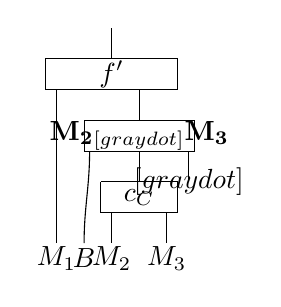
\begin{tikzpicture}[yscale=0.78, xscale=0.7]
\draw (2,2.5) -- (2,3);
\draw (0.8,2) -- (3.2,2) -- (3.2,2.5) -- (0.8,2.5) -- (0.8,2);
\node at (2,2.25) {$f'$};
\draw (1,2) -- (1,-0.5);
\draw (2.5,2) -- (2.5,1.5);
\draw (1.5,1.5) -- (3.5,1.5) -- (3.5,1) -- (1.5,1) -- (1.5,1.5);
\node at (2.5,1.25) {${\bf M_2}_{\tinydot[gray dot]}{\bf M_3}$};
\draw (2.5,1) -- (2.5,0.5);
\draw (1.6,1) to [in=90,out=-90] (1.5,-0.5);
\draw (3.4,1) to (3.4,0.5); 
\node at (3.4,0.5) {$\tinydot[gray dot]$};
\draw (2,0) to (2,-0.5);
\draw (3,0) to (3,-0.5);
\draw (1.8, 0.5) -- (3.2,0.5) -- (3.2,0) -- (1.8,0) -- (1.8,0.5);
\node at (2.5,0.25) {$c_C$};
\node at (1.5,-0.75) {$B$};
\node at (1,-0.75) {$M_1$};
\node at (2,-0.75) {$M_2$};
\node at (3,-0.75) {$M_3$};
\end{tikzpicture}
\end{aligned}
\end{equation}
The first equality is obtained by interchanging $c_C$ and ${\bf M_1} \hor \mathid$, the second holds because $f$ is a cocone of $_{\tinydot [gray dot]}{\bf M_1} \hor \mathid_{M_2} \hor \mathid_{M_3}$ and $\mathid_{M_1} \hor { \bf M_2}_{\tinydot [gray dot]} \hor \mathid_{M_3}$, the third since $f= f' \ver (\mathid \hor c_C)$, and the fourth by definition of ${\bf M_2}_{\tinydot[gray dot]}{\bf M_3}$. This means that there exists a morphism $f''$ such that $f= f' \ver (\mathid \hor c_C) = f'' \ver \tilde{c}_B \ver (\mathid \hor c_C)$, hence $f$ factorizes through $\pi_1$. A similar argument shows that $\pi_2$ is a coequaliser as well. 

The components of the {\bf left unitor} $l_{\bf M}: U_A \ominus {\bf M} \rightarrow {\bf M}$ are given by $(\mathid, l_{M}, \mathid)$, where $ l_{M}$ is defined as follows: By the module laws, ${\bf M}_{\tinydot[gray dot]}: A \hor M \rightarrow M$ is a coequaliser of the maps $_{\tinydot[gray dot]}{\bf A} \hor \mathid_{M}$ and $\mathid_{A} \hor {\bf M}_{\tinydot[gray dot]}$. The canonical isomorphisms between ${\bf M}$ and ${\bf A}_{\tinydot[gray dot]}{\bf M}$ is the middle component of $l_{\bf M}$, and naturality of $l$ follows from commutativity of the diagram below. We can define $r$, and prove its naturality, in a similar way.
    
\begin{tikzpicture}[xscale=4,yscale=2]
 \node (tl) at (0,1) {$A \hor A \hor M$};
 \node (bl) at (0,0) {$B \hor B \hor N$};
  \node (tm) at (1,1) {$A \hor M$};
 \node (bm) at (1,0) {$B \hor N$};
\draw[->] ([yshift=1.5pt] tl.east) to node[above] {${}_{\tinydot[gray dot]}U_{A} \hor \mathid_M$} ([yshift=1.5pt] tm.west);
\draw[->] ([yshift=-1.5pt] tl.east) to node[below] {$\mathid_{A} \hor {\bf M}_{\tinydot[gray dot]}$} ([yshift=-1.5pt] tm.west);
\draw[->] ([yshift=1.5pt] bl.east) to node[above] {$_{\tinydot[gray dot]}U_A \hor \mathid_N$} ([yshift=1.5pt] bm.west);
\draw[->] ([yshift=-1.5pt] bl.east) to node[below] {$\mathid_{B} \hor {N}_{\tinydot[gray dot]}$} ([yshift=-1.5pt] bm.west);
 \node (r1) at (2,1.25) {$A_{\tinydot[gray dot]} M$};
 \node (r2) at (1.6,0.75) {$M$};
  \node (r3) at (2,0.25) {$B_{\tinydot[gray dot]} N$};
 \node (r4) at (1.6,-0.25) {$N$};
 \draw[->] (tm) to node[above] {$c_M$} (r1.west);
 \draw[->] (tm) to node[below] {${\bf M}_{\tinydot[gray dot]}$} (r2);
  \draw[->] (bm) to node[above] {$c_N$} (r3.west);
 \draw[->] (bm) to node[below] {${\bf N}_{\tinydot[gray dot]}$} (r4);
  \draw[->, dashed] (r1) to node[left] {$l_M$} (r2);
 \draw[->, dashed] (r3) to node[right] {$l_N$} (r4);
  \draw[->, dashed] (r1) to node[right] {$f \tinydot[gray dot] g$} (r3);
 \draw[->, dashed, cross] (r2) to node[left, yshift=10pt] {$g$} (r4);
 \draw[->] (tl) to node[left] {$f \hor f \hor g$} (bl);
 \draw[->] (tm) to node[left] {$f \hor g$} (bm);
\end{tikzpicture}
\end{proof}


\subsection{The braided monoidal structure of $\Alg$}\label{sec:brmonDalg}

In this section we will prove that $\Alg$ is a symmetric monoidal double category

\begin{prop}\label{lem:algsymmon}
Let {\bf B} be a (braided/symmetric) monoidal category, the double category $\Alg({\cat B})$ of algebras, bimodules and bimodule homomorphisms in {\bf B} is (braided/symmetric) monoidal
\end{prop}

\begin{proof}

We have seen that $\D_0$ and $\D_1$ are (braided/symmetric) monoidal. Clearly, $S$ and $T$ are strict monoidal functors preserving the associativity and unit constraints, and $U_I$ is the monoidal unit of $D_1$, when $I$ is the monoidal unit of $D_0$.

Unfolding definitions shows that the globular isomorphism $\fu$ from $U \circ \tens$ to $\tens \circ (U \times U)$ is the identity. We define the exchange law, ${\bf \fx}$, between the functors $\ominus$ and $\tens$ as $(\mathid, \xi, \mathid)$, where $\xi$ is the unique morphism completing the commuting diagram below.
In this diagram, $c$, $c_M$, and $c_N$ are the coequalisers defining  $({M_1} \hor {N_1})_{\tinydot[gray dot]}({M_2} \hor {N_2})$, ${M_1}_{\tinydot[gray dot]} M_2$, and ${N_1}_{\tinydot[gray dot]} N_2$, respectively. By a similar argument given while defining the associator ${\bf a}$ for the double category, one can show that $c_M \hor c_N$ is the coequaliser of the lower two parallel maps in the diagram. The two leftmost vertical morphisms are natural isomorphisms witnessing the exchange law between the tensor product and horizontal composition. The middle morphism plays a role in the rest of this proof, for convenience we will give it the name $\hat{\sigma}$.

\begin{equation}\label{def:xi}
  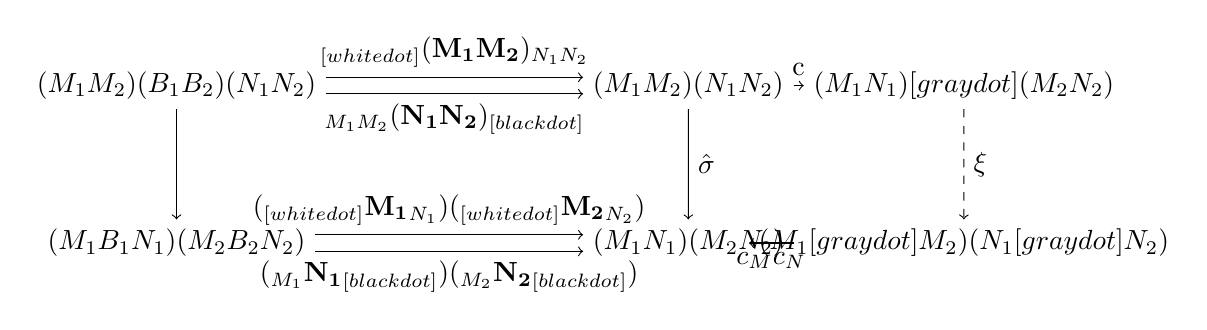
\begin{tikzpicture}[xscale=5, yscale=2, thin]
    \node (tl) at (-.3,1) {$(M_1 \tens M_2) \hor (B_1 \tens B_2) \hor (N_1 \tens N_2)$};
    \node (bl) at (-.3,0) {$(M_1 \hor B_1 \hor N_1) \tens (M_2 \hor B_2 \hor N_2)$};
    \node (t) at (1,1) {$(M_1 \tens M_2) \hor (N_1 \tens N_2)$};
    \node (b) at (1,0) {$(M_1 \hor N_1) \tens (M_2 \hor N_2)$};
    \node (tr) at (1.7,1) {$({M_1} \tens {N_1}) \tinydot[gray dot] ({M_2} \tens {N_2})$};
    \node (br) at (1.7,0) {$({M_1} \tinydot[gray dot] {M_2}) \tens ({N_1} \tinydot[gray dot] {N_2})$};
    \draw[->] (tl) to node[left] {$\iso$} (bl);
    \draw[->] (t) to node[right] {$\iso \hat{\sigma} $} (b);
    \draw[->, dashed] (tr) to node[right] {$\iso {\xi} $} (br);
    \draw[->] (t) to node[above] {c} (tr);
    \draw[->] (b) to node[below] {$c_M \tens c_N$} (br);
    \draw[->] ([yshift=1.5pt]tl.east) to node[above] {${}_{\tinydot[white dot]}(\mathbf{M_1} \tens \mathbf{M_2}) \hor \mathid_{N_1 \tens N_2}$} ([yshift=1.5pt]t.west);
    \draw[->] ([yshift=-1.5pt]tl.east) to node[below] {$\mathid_{M_1 \tens M_2} \hor (\mathbf{N_1} \tens \mathbf{N_2})_{\tinydot[black dot]}$} ([yshift=-1.5pt]t.west);
    \draw[->] ([yshift=1.5pt]bl.east) to node[above] {$
    ({}_{\tinydot[white dot]}\mathbf{M_1} \hor \mathid_{N_1}) \tens ({}_{\tinydot[white dot]}\mathbf{M_2} \hor \mathid_{N_2})$} ([yshift=1.5pt]b.west);
    \draw[->] ([yshift=-1.5pt]bl.east) to node[below] {$(\mathid_{M_1} \hor \mathbf{N_1}_{\tinydot[black dot]}) \tens (\mathid_{M_2} \hor \mathbf{N_2}_{\tinydot[black dot]})$} ([yshift=-1.5pt]b.west);
  \end{tikzpicture}
 \end{equation}


What is left to prove is that the diagrams given in points (iv),(v),(vi), and (ix) of Definition ~\ref{def:symmondoub} commute. Because $\fu$ and $\fx$ are globular, it suffices to verify commutativity of the diagrams only for the middle components of the extended module homomorphisms.

The first equation of (iv) corresponds to the front square of the diagram below. The unlabelled arrows represent the coequalisers defining their target object.
The bottom square and the upper right square commute by the definition of $\xi$. The square at the back commutes  by coherence of the bicategory ${\cat B}$ and the pseudofunctor $\tens$. The upper left and lower right square commute by definition of ${\bf a}$. The lower left and the top square commute by definition of $\tinydot[gray dot]$ and $\xi$.
It follows that the front square must commute as well.
\begin{equation}
\begin{tikzpicture}[xscale=3.2, yscale=2]
%lowersquare
\node (b1) at (0,0) [] {$(M_1 \tens N_1) \hor ((M_2 \hor M_3) \tens (N_2 \hor N_3))$};
\node (b2) at (2,0) [] {$(M_1 \hor (M_2 \hor M_3) \tens (N_1 \hor (N_2 \hor N_3))$};
\node (b3) at (1,-0.5) [] {$(M_1 \tens {N_1})_{\tinydot[gray dot]} (({M_2}_{\tinydot[gray dot]} M_3) \tens ({N_2}_{\tinydot[gray dot]} N_3))$};
\node (b4) at (3,-0.5) [] {$({M_1}_{\tinydot[gray dot]} ({M_2}_{\tinydot[gray dot]} M_3 )) \tens ({N_1}_{\tinydot[gray dot]} ({N_2}_{\tinydot[gray dot]} N_3))$}; 
\draw[->] (b1) to node[above, xshift=7pt] {$\hat{\sigma}$} (b2);
\draw[->] (b3) to node[above] {$\xi$} (b4);
\draw[->] (b1) to node[above] {} (b3); 
\draw[->] (b2) to node[above] {} (b4);
%middlesquare
\node (m1) at (0,1.5) [] {$(M_1 \tens N_1) \hor ((M_2 \tens N_2)) \hor (M_3 \tens N_3))$};
\node (m2) at (2,1.5) [] {$((M_1 \hor M_2) \hor M_3) \tens ((N_1 \hor N_2) \hor N_3)$};
\node (m3) at (1,1) [] {$(M_1 \tens {N_1})_{\tinydot[gray dot]} ((M_2 \tens {N_2})_{\tinydot[gray dot]} (M_3 \tens N_3))$};
\node (m4) at (3,1) [] {$({M_1}_{\tinydot[gray dot]} {M_2})_{\tinydot[gray dot]} {M_3}) \tens (({N_1}_{\tinydot[gray dot]}N_2)_{\tinydot[gray dot]} N_3)$};
\draw[->] (m1) to node[above] {} (m3); 
\draw[->] (m2) to node[above] {} (m4);
%lowervertical
\draw[->] (m1) to node[left] {$\mathid \hor \hat{\sigma}$} (b1); 
\draw[->] (m2) to node[left] {$\alpha \tens \alpha$} (b2);
\draw[->, cross] (m3) to node[left, yshift=8pt] {$\mathid \tinydot[gray dot] \xi$} (b3); 
\draw[->] (m4) to node[left] {$a \tens a$} (b4);
%uppersquare
\node (u1) at (0,3) [] {$((M_1 \tens N_1) \hor (M_2 \tens N_2)) \hor (M_3 \tens N_3)$};
\node (u2) at (2,3) [] {$((M_1 \hor M_2) \tens (N_1 \hor N_2)) \hor (M_3 \tens N_3)$};
\node (u3) at (1,2.5) [] {$((M_1 \tens N_1)_{\tinydot[gray dot]}(M_2 \tens N_2))_{\tinydot[gray dot]}(M_3 \tens N_3)$};
\node (u4) at (3,2.5) [] {$(({M_1}_{\tinydot[gray dot]} M_2) \tens ({N_1}_{\tinydot[gray dot]} N_2))_{\tinydot[gray dot]} (M_3 \tens N_3)$};
\draw[->] (u1) to node[left] {$\alpha$} (m1); 
\draw[->] (u2) to node[left] {$\hat{\sigma}$} (m2);
\draw[->, cross] (u3) to node[left] {$a$} (m3); 
\draw[->] (u4) to node[left] {$\xi$} (m4);
\draw[->, cross] (u3) to node[above, xshift=8pt] {$\xi_{\tinydot[gray dot]} \mathid$} (u4); 
\draw[->] (u1) to node[above] {$\hat{\sigma} \hor \mathid$} (u2);
\draw[->] (u1) to node[below] {} (u3); 
\draw[->, cross] (u2) to node[above] {} (u4);
\end{tikzpicture}
\end{equation}

All other equations concerning $\xi$ are proven in the same way. These are the second and third equation of (iv), the first equation of (v), the first and the third equation of (vi), and the first equation of (ix).
It is easy to see that equations concerning $\fu$ hold, keeping in mind that $\fu$ is the identity, and $U_{\alpha_{A,B,C}} = \alpha_{U_A,U_B,U_C}$, $U(\rho_A) = \rho_{U_A}$, $U(\lambda_A) = \lambda_{U_A}$, and $\sigma_{U_A,U_B} = U(\sigma_{A,B})$.
These remaining equations are the second equation of (v), the second and the fourth equation of (vi), and the second equation of (ix).
\end{proof}

\begin{equation*}
\mbox{[Updated until here]}
\end{equation*}

\subsection{Companions and conjoints in $\Alg$}\label{sec:fibDalg}
Finally, we will prove that $\Alg(\cat B$) is fibrant. this is the last step we need to take to show that we can lift $\Alg({\cat B})$ to obtain the bicategory ${\cA}lg({\cat B})$, which preserves any braided monoidal structure.

\begin{lem}\label{lem:algfib}
The double category $\Alg({\cat B})$ is fibrant.
\end{lem}

\begin{proof}
Let $f$ be a morphism of ${\lD_1}$. The companion of $f$ is defined by the following data: 

\begin{equation}\label{eq:companion}
\hat{f}:= 
\begin{aligned}
 \begin{tikzpicture}[scale=0.6] 
\draw (0.5,-0.5)node[below]{$A$} -- (0.5, -0.2);
\draw (0.2,-0.2) -- (0.8,-0.2) -- (0.8,0.7) -- (0.2,0.7) -- (0.2,-0.2);
\draw (0.5,0.7) to[out=90,in=160] (1.2,1.2) node[gray dot] {};
\draw (1.2,-0.5) node[below]{$B$} to (1.2,1.2);
\draw (1.9,0.7) to[out=90, in=20] (1.2,1.2){};
\draw (1.9,0.7)  to (1.9,-0.5)node [below]{$B$};
\draw (1.2,1.9) -- (1.2,1.2){};
\node at (0.5,0.25)[] {$f$};
\node at (1.2,2.1)[]{$B$};
\end{tikzpicture}
\end{aligned}
\quad \quad \eta_{\hat{f}} := (id_A, f, f)
\quad \quad \epsilon_{\hat{f}} := (f, \mathid_B, \mathid_B)
\end{equation}

The first equation of ~\ref{eq:compeqn} holds because $\epsilon_{\hat{f}} \circ \eta_{\hat{f}} = (f,f,f) = U_f$. The left-hand-side of the second equation corresponds to $\eta_{\hat{f}} \ominus \epsilon_{\hat{f}}= (id_A, f\tinydot[gray dot] \mathid_B, \mathid_B)$, where $f\tinydot[gray dot] \mathid_B: {U_A}_{\tinydot[gray dot]} \hat{f} \rightarrow \hat{f}_{\tinydot[gray dot]}U_B$ is the unique map that makes back of the diagram below commute.  We need to show that this equals $1_{\hat{f}} = (\mathid_A, \mathid_B, \mathid_B)$.

\begin{tikzpicture}[xscale=4,yscale=2]
 \node (tl) at (0,1) {$A \hor A \hor B$};
 \node (bl) at (0,0) {$B \hor B \hor B$};
  \node (tm) at (1,1) {$A \hor B$};
 \node (bm) at (1,0) {$B \hor B$};
\draw[->] ([yshift=1.5pt] tl.east) to node[above] {${}_{\tinydot[white dot]}U_A \hor \mathid_B$} ([yshift=1.5pt] tm.west);
\draw[->] ([yshift=-1.5pt] tl.east) to node[below] {$\mathid_{A} \hor \hat{f}_{\tinydot[gray dot]}$} ([yshift=-1.5pt] tm.west);
\draw[->] ([yshift=1.5pt] bl.east) to node[above] {$_{\tinydot[white dot]}\hat{f} \hor \mathid_B$} ([yshift=1.5pt] bm.west);
\draw[->] ([yshift=-1.5pt] bl.east) to node[below] {$\mathid_{B} \hor {U_B}_{\tinydot[gray dot]}$} ([yshift=-1.5pt] bm.west);
 \node (r1) at (2,1.25) {$A_{\tinydot[gray dot]} B$};
 \node (r2) at (1.6,0.75) {$B$};
  \node (r3) at (2,0.25) {$B_{\tinydot[gray dot]} B$};
 \node (r4) at (1.6,-0.25) {$B$};
 \draw[->] (tm) to node[above] {$c_A$} (r1.west);
 \draw[->] (tm) to node[below] {$\hat{f}_{\tinydot[gray dot]}$} (r2);
  \draw[->] (bm) to node[above,xshift=-4pt] {$c_B$} (r3.west);
 \draw[->] (bm) to node[below] {$_{\tinydot[white dot]}\hat{f}$} (r4);
  \draw[->, dashed] (r1) to node[left] {$l_{\hat{f}}$} (r2);
 \draw[->, dashed] (r3) to node[right] {$r_{\hat{f}}$} (r4);
  \draw[->, dashed] (r1) to node[right] {$f \tinydot[gray dot] \mathid_B$} (r3);
 \draw[->, dashed, cross] (r2) to node[right,yshift=7pt] {$\mathid_B$} (r4);
 \draw[->] (tl) to node[left] {$f \hor f \hor \mathid_B$} (bl);
 \draw[->] (tm) to node[left] {$f \hor \mathid_B$} (bm);
\end{tikzpicture}

In this diagram, $c_A$ and $c_B$ are the coequalisers defining ${U_A}_{\tinydot[gray dot]} \hat{f}$ and $\hat{f}_{\tinydot[gray dot]}U_B$, respectively.
It is easy to check that $\hat{f}_{\tinydot[gray dot]}$ and $_{\tinydot[white dot]}{\hat{f}}$ are coequalisers as well. The morphisms $B$, $l_{\hat{f}}$ and $r_{\hat{f}}$ are the unique morphisms that make all diagrams commute. If we assume the double category to be strict, it follows that $f \tinydot[gray dot] \mathid_B = \mathid_B$, and thus $\eta_{\hat{f}} \ominus \epsilon_{\hat{f}} = 1_{\hat{f}}$.

This simultaneously proves that $f$ has a conjoint, because $\Alg({\bf C}^{h* op}) \cong$ $\Alg({\cat C})$.
\end{proof}

\begin{eg}
When we take the category $\mathcal{A}B$ of Abelian groups and group homomorphisms as our symmetric monoidal category, we obtain the double category $\cMod$ of rings, ring homomorphisms, bimodules and bimodule homomorphisms. As a consequence of Lemma's ~\ref{lem:algdouble}, ~\ref{lem:algsymmon}, and ~\ref{lem:algfib}, and Theorem ~\ref{thm:lcbcfunctor}, the horizontal bicategory $\cMod$ of $\lMod$ is a symmetric monoidal.
\end{eg}

\begin{thm}\label{thm:eqcomp}
Let {\bf C} be a braided monoidal category where all coequalisers exist and where the tensor product preserves coequalisers. The loose bicategory $\mathcal{A}lg({\cat C})$ is braided monoidal; it is symmetric whenever {\bf C} is symmetric.
\end{thm}

\begin{proof}
By $\ref{lem:algdouble}, \ref{lem:algsymmon}, \ref{lem:algfib}$, $\mathbb{Alg}({\bf C})$ is braided monoidal and Fibrant; and it is symmetric or sylleptic whenever {\bf C} is symmetric or sylleptic, respectively. As a result, all constraints have loosely strong companions.  Therefore we may apply Theorem ~\ref{thm:lcbcfunctor} to finish the proof.
\end{proof}

\subsection{Monoidal Functors and Transformations}
We extend $\bAlg$ to functors and transformations and show that it gives rise to a pseudo functor. 
\begin{prop}\label{prop:mfunctor}
Any braided monoidal strong functor $F: {\bf C} \rightarrow {\bf D}$ which preserves coequalisers lifts to a braided monoidal strong double functor $\bAlg{F}:  \bAlg{\bf C} \rightarrow \bAlg{ \bf D}$. The functor $\bAlg{F}$ is sylleptic or symmetric, whenever $F$ is sylleptic or symmetric, respectively.
\end{prop}

\begin{proof}
Any braided monoidal functor preserves algebras and bimodules. The functor $\bAlg(F)_0$ maps an algebra $(A, \tinymult[gray dot], \tinyunit[gray dot])$ to the algebra $(FA, F(\tinymult[gray dot])\circ \chi, F(\tinyunit[gray dot])\circ \iota)$. The functor $\bAlg(F)_1$ maps an A-B-bimodule {\bf M} to $F({\bf M}) \circ \chi_{A, M \otimes B} \circ (\id \otimes \chi_{M,B)}$. On extended bimodule homomorphisms $\bAlg$ is defined componentwise. 
The pseudo double transformation $F_{\odot}$ is the unique morphism defined by the coequalisers below.

\begin{equation}\label{def:xi}
  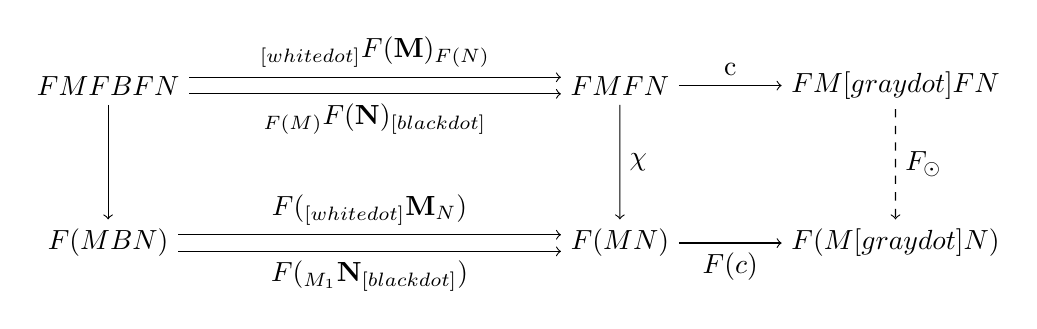
\begin{tikzpicture}[xscale=5, yscale=2, thin]
    \node (tl) at (-.3,1) {$FM \ten FB \ten FN$};
    \node (bl) at (-.3,0) {$F(M \ten B \ten N)$};
    \node (t) at (1,1) {$FM \ten FN$};
    \node (b) at (1,0) {$F(M\ten N)$};
    \node (tr) at (1.7,1) {$FM \tinydot[gray dot] FN$};
    \node (br) at (1.7,0) {$F(M \tinydot[gray dot] N)$};
    \draw[->] (tl) to node[left] {$\iso$} (bl);
    \draw[->] (t) to node[right] {$\chi \iso$} (b);
    \draw[->, dashed] (tr) to node[right] {$F_{\odot}$} (br);
    \draw[->] (t) to node[above] {c} (tr);
    \draw[->] (b) to node[below] {$F(c)$} (br);
    \draw[->] ([yshift=1.5pt]tl.east) to node[above] {${}_{\tinydot[white dot]}F(\mathbf{M})  \ten \mathid_{F(N)}$} ([yshift=1.5pt]t.west);
    \draw[->] ([yshift=-1.5pt]tl.east) to node[below] {$\mathid_{F(M)} \ten F(\mathbf{N})_{\tinydot[black dot]}$} ([yshift=-1.5pt]t.west);
    \draw[->] ([yshift=1.5pt]bl.east) to node[above] {$
    F({}_{\tinydot[white dot]}\mathbf{M} \tens \mathid_{N} )$} ([yshift=1.5pt]b.west);
    \draw[->] ([yshift=-1.5pt]bl.east) to node[below] {$F(\mathid_{M_1} \ten \mathbf{N}_{\tinydot[black dot]})$} ([yshift=-1.5pt]b.west);
  \end{tikzpicture}
 \end{equation}


The two commuting diagrams below show that $F_{\odot}$ is a module homomorphism and that $F_{\odot}$ is natural in $\mathbb{A}lg{\bf D}_1$.

\begin{equation}
\begin{tikzpicture}[xscale=2.5, yscale=2]
%uppersquare
\node (u1) at (1,3) [] {$F(A\otimes M \otimes N \otimes C)$};
\node (u2) at (3,3) [] {$F(A \otimes M \tinydot[gray dot] N \otimes C)$};
\node (u3) at (0,2.5) [] {$FA \ten FM \otimes FN \ten FC$};
\node (u4) at (2,2.5) [] {$FA \ten FM \tinydot[gray dot]FM \ten FC $};
\node (u-1) at (-1,3) [] {$F(A\otimes M \otimes B \ten N \otimes C)$};
\node (u-3) at (-2,2.5) [] {$FA \ten FM \otimes FB \ten FN \ten FC$};
%leftuppersquare
\draw[->] ([yshift=1.5pt]u-1.east) to node[above] {} ([yshift=1.5pt]u1.west);
    \draw[->] ([yshift=-1.5pt]u-1.east) to node[below] {} ([yshift=-1.5pt]u1.west);
        \draw[->] (u-3) to (u-1); 
 %%%   
\draw[->] (u1) to node[above] {} (u2);
\draw[->] (u3) to node[below] {} (u1); 
\draw[->, dashed ] (u4) to node[] {$\mathid \ten F_{\odot} \ten \mathid$} (u2);
%lowersquare
\node (m1) at (1,1.5) [] {$F(M \otimes N )$};
\node (m2) at (3,1.5) [] {$F(M \tinydot[gray dot] N) $};
\node (m3) at (0,1) [] {$FM \ten FN$};
\node (m4) at (2,1) [] {$FM \tinydot[gray dot] FN$};
\draw[->] (m3) to node[above] {} (m1); 
\draw[->, dashed] (m4) to node[] {$F_{\odot}$} (m2);
\draw[->] (m3) to node[above, xshift=8pt] {} (m4); 
\draw[->] (m1) to node[above] {} (m2);
\node (m-1) at (-1,1.5) [] {$F( M \ten B \ten N)$};
\node (m-3) at (-2,1) [] {$FM \ten  FB \ten FN $};
%leftlowersquare
\draw[->] ([yshift=1.5pt]m-1.east) to node[above] {} ([yshift=1.5pt]m1.west);
    \draw[->] ([yshift=-1.5pt]m-1.east) to node[below] {} ([yshift=-1.5pt]m1.west);
 \draw[->] ([yshift=1.5pt]m-3.east) to node[above] {} ([yshift=1.5pt]m3.west);
    \draw[->] ([yshift=-1.5pt]m-3.east) to node[below] {} ([yshift=-1.5pt]m3.west);
    \draw[->] (m-3) to (m-1);
%vertical
\draw[->] (u1) to node[] {$F({\bf M}_{\tinydot[gray dot]} \ten  {}_{\tinydot[gray dot]}{\bf N})$} (m1); 
\draw[->, dashed] (u2) to node[] {$F({\bf M}\tinydot[gray dot]{\bf N})$} (m2);
\draw[->, cross] (u3) to node[] {$F({\bf M})_{\tinydot[gray dot]} \ten {}_{\tinydot[gray dot]}F({\bf N})$} (m3); 
\draw[->, cross, dashed] (u4) to node[] {$F{\bf M }\tinydot[gray dot] F{\bf N}$} (m4);
\draw[->] (u-1) to node[] {$F({\bf M}_{\tinydot[gray dot]} \ten \mathid_B \ten {}_{\tinydot[gray dot]}{\bf N})$} (m-1);
\draw[->] (u-3) to node[above] {$F({\bf M})_{\tinydot[gray dot]} \ten \mathid_{FB} \ten {}_{\tinydot[gray dot]}F({\bf N})$} (m-3);
%%%% cross
\draw[->, cross] ([yshift=1.5pt]u-3.east) to node[above] {} ([yshift=1.5pt]u3.west);
    \draw[->, cross] ([yshift=-1.5pt]u-3.east) to node[below] {} ([yshift=-1.5pt]u3.west);
    \draw[->, cross] (u3) to node[above, xshift=8pt] {} (u4); 
\end{tikzpicture}
\end{equation}

\begin{equation}
\begin{tikzpicture}[xscale=2.5, yscale=2]
%uppersquare
\node (u1) at (1,3) [] {$F(M \otimes N)$};
\node (u2) at (3,3) [] {$F(M \tinydot[gray dot] N )$};
\node (u3) at (0,2.5) [] {$ FM \otimes FN $};
\node (u4) at (2,2.5) [] {$FM \tinydot[gray dot] FM$};
\node (u-1) at (-1,3) [] {$F(M \otimes B \ten N)$};
\node (u-3) at (-2,2.5) [] {$FM \otimes FB \ten FN$};
%leftuppersquare
\draw[->] ([yshift=1.5pt]u-1.east) to node[above] {} ([yshift=1.5pt]u1.west);
    \draw[->] ([yshift=-1.5pt]u-1.east) to node[below] {} ([yshift=-1.5pt]u1.west);
        \draw[->] (u-3) to (u-1); 
 %%%   
\draw[->] (u1) to node[above] {} (u2);
\draw[->] (u3) to node[below] {} (u1); 
\draw[->, dashed ] (u4) to node[] {$ F_{\odot}$} (u2);
%lowersquare
\node (m1) at (1,1.5) [] {$F(M' \otimes N' )$};
\node (m2) at (3,1.5) [] {$F(M' \tinydot[gray dot] N') $};
\node (m3) at (0,1) [] {$FM' \ten FN'$};
\node (m4) at (2,1) [] {$FM' \tinydot[gray dot] FN'$};
\draw[->] (m3) to node[above] {} (m1); 
\draw[->, dashed] (m4) to node[] {$F_{\odot}$} (m2);
\draw[->] (m3) to node[above, xshift=8pt] {} (m4); 
\draw[->] (m1) to node[above] {} (m2);
\node (m-1) at (-1,1.5) [] {$F(M' \ten B \ten N')$};
\node (m-3) at (-2,1) [] {$FM' \ten  FB \ten FN' $};
%leftlowersquare
\draw[->] ([yshift=1.5pt]m-1.east) to node[above] {} ([yshift=1.5pt]m1.west);
    \draw[->] ([yshift=-1.5pt]m-1.east) to node[below] {} ([yshift=-1.5pt]m1.west);
 \draw[->] ([yshift=1.5pt]m-3.east) to node[above] {} ([yshift=1.5pt]m3.west);
    \draw[->] ([yshift=-1.5pt]m-3.east) to node[below] {} ([yshift=-1.5pt]m3.west);
    \draw[->] (m-3) to (m-1);
%vertical
\draw[->] (u1) to node[] {$F(f \ten g)$} (m1); 
\draw[->, dashed] (u2) to node[] {$F(f \tinydot[gray dot] g)$} (m2);
\draw[->, cross] (u3) to node[] {$F(f) \ten F(g)$} (m3); 
\draw[->, cross, dashed] (u4) to node[] {$F(f) \tinydot[gray dot] F(g)$} (m4);
\draw[->] (u-1) to node[] {$F(f \ten \mathid \ten g)$} (m-1);
\draw[->] (u-3) to node[above] {$F(f) \ten \mathid \ten F(g)$} (m-3);
%%%% cross
\draw[->, cross] ([yshift=1.5pt]u-3.east) to node[above] {} ([yshift=1.5pt]u3.west);
    \draw[->, cross] ([yshift=-1.5pt]u-3.east) to node[below] {} ([yshift=-1.5pt]u3.west);
    \draw[->, cross] (u3) to node[above, xshift=8pt] {} (u4); 
\end{tikzpicture}
\end{equation}

One can show with a similar commuting diagram that $F_{\odot}$ is a natural isomorphism in $\mathbb{A}lg({\bf D})$.
The natural isomorphism $F_U: U_{F_0(A)} \rightarrow F_1(U_A)$ is a strict identity, by the definition of $U, \mathbb{A}lgF_0$, and $\mathbb{A}lgF_1$. Finally, it is straightforward that $S \circ F_1 = F_0 \circ S$ and $T \circ F_1 = F_0 \circ T$.

It remains to prove that the double functor $\mathbb{A}lgF$ is braided monoidal strong and sylleptic or symmetric whenever $F$ is sylleptic or symmetric. The first condition i) is that $F_0$ and $F_1$ are braided monoidal strong functors, which comes down to showing that the natural transformations $\chi: \ten (F,F) \rightarrow  F\ten$ and $`\iota: I_{\cD} \rightarrow F(I_{\cC})$ give rise to tight transformations of double categories, whose components are well-defined as algebra and module homomorphisms, respectively. This follows from naturality of $\chi$, and coherence and functoriality of $F$. Coherence of $\mathbb{A}lgF_0$ and $\mathbb{A}lgF_1$ follows from coherence of $F$. Similarly, the sylleptic or symmetric monoidal structure of $F$, gives rise to a sylleptic or symmetric monoidal structure for $F_0$, $F_1$. For condition ii) we need to show that $F_0 \circ S$ equals $S \circ F_1$ as monoidal functors, and similarly, $F_0 \circ T = T \circ F_1$. The first equality amounts to  $\chi^{F_0 \circ S} = \chi^{S \circ F_1}$ and $\chi^{F_0 \circ S} = \chi^{S \circ F_1}$, where we have written the functor that $\phi$ belongs to in superscript. Unfolding definitions gives us $F_0(\chi^{S}) \circ \chi^{F_0} = S(\chi^{F_1}) \circ \chi^{S}$. This holds, since $\chi^S$ is the identity. The constraints are shown to hold in a similar way.

Finally, the first of the two additional diagrams given in condition (iii) of ~\ref{def:monfunc} corresponds to the front square of the commuting diagram below. The unlabelled arrows represent the coequalisers defining their target object. The back square commutes by coherence of $F$. The squares on the sides commute by definition of $\xi$, $F_{\odot}$, and $\chi \tinydot[gray dot] \chi$ and by naturality of $\chi$. It follows that the fron square must commute.The second diagram can be shown to hold by a similar commuting diagram.



\begin{equation}
\begin{tikzpicture}[xscale=3.2, yscale=2]
%lowersquare
\node (b1) at (0,0) [] {$F((N\ten L) \ten (M \ten K))$};
\node (b2) at (2,0) [] {$F((N \ten M) \ten (L \ten K))$};
\node (b3) at (1,-0.5) [] {$F((N\ten L) \tinydot[gray dot] (M \ten K))$};
\node (b4) at (3,-0.5) [] {$F((N \tinydot[gray dot] M) \ten (L \tinydot[gray dot] K))$}; 
\draw[->] (b1) to node[above, xshift=12pt] {$F(\hat{\sigma})$} (b2);
\draw[->] (b3) to node[above] {$F(\xi)$} (b4);
\draw[->] (b1) to node[above] {} (b3); 
\draw[->] (b2) to node[above] {} (b4);
%middlesquare
\node (m1) at (0,1.5) [] {$F(N\ten L) \ten F(M \ten K)$};
\node (m2) at (2,1.5) [] {$F(N \ten M) \ten F(L \ten K)$};
\node (m3) at (1,1) [] {$F(N\ten L) \tinydot[gray dot] F(M \ten K)$};
\node (m4) at (3,1) [] {$F(N \tinydot[gray dot] M) \ten F(L \tinydot[gray dot] K)$};
\draw[->] (m1) to node[above] {} (m3); 
\draw[->] (m2) to node[above] {} (m4);
%lowervertical
\draw[->] (m1) to node[left] {$\chi$} (b1); 
\draw[->] (m2) to node[left] {$\chi$} (b2);
\draw[->, cross] (m3) to node[left, yshift=8pt] {$F_{\odot}$} (b3); 
\draw[->] (m4) to node[left] {$\chi$} (b4);
%uppersquare
\node (u1) at (0,3) [] {$(FN \ten FL) \ten (FM \ten FK)$};
\node (u2) at (2,3) [] {$(FN \ten FM) \ten (FL \ten FK)$};
\node (u3) at (1,2.5) [] {$(FN \ten FL) \tinydot[gray dot] (FM \ten FK)$};
\node (u4) at (3,2.5) [] {$(FN \tinydot[gray dot] FM) \ten (FL \tinydot[gray dot] FK)$};
\draw[->] (u1) to node[left] {$\chi \ten \chi$} (m1); 
\draw[->] (u2) to node[left] {$\chi \ten \chi$} (m2);
\draw[->, cross] (u3) to node[left] {$\chi \tinydot[gray dot] \chi$} (m3); 
\draw[->] (u4) to node[left] {$F_{\odot} \ten F_{\odot}$} (m4);
\draw[->, cross] (u3) to node[above, xshift=8pt] {$\xi$} (u4); 
\draw[->] (u1) to node[above] {$\hat{\sigma}$} (u2);
\draw[->] (u1) to node[below] {} (u3); 
\draw[->, cross] (u2) to node[above] {} (u4);
\end{tikzpicture}
\end{equation}
\end{proof}  



Note that a similar result does not hold for braided monoidal lax or oplax functors, as the transformations $\chi$ and $\iota$ of $\mathbb{A}lg(F)$ may not have loosely strong companions. 

\begin{prop}\label{prop:mtrans}
Let $F,G: {\bf C} \rightarrow {\bf D}$ be braided monoidal functors that preserve coequalisers. A braided monoidal transformation $\alpha: F \Rightarrow G$ lifts to a braided monoidal double transformation $\bAlg \alpha: \bAlg F \Rightarrow \bAlg G$. Furthermore, $\bAlg \alpha$ is sylleptic or symmetric, whenever $\alpha$ is sylleptic or symmetric, respectively.
\end{prop}

\begin{proof}
The components of any monoidal transformation $\alpha$ are algebra homomorphisms by the two coherence equations and by naturality of $\alpha$; hence, $\alpha$ gives rise to a natural transformation $\bAlg \alpha_0: \bAlg F_0 \Rightarrow \bAlg G_0$.
It gives rise to a natural transformation $\bAlg \alpha_1: \bAlg F_1 \Rightarrow \bAlg  G_1$, where the component $\alpha_{\bf M}$ of an $A-B-$Bimodule ${\bf M}$ is defined as $(\alpha_A, \alpha_M, \alpha_B)$. This is well-defined by naturality of $\alpha$ and the coherence equations for monoidal transformations.

The first equality for tight transformation follows from the first coherence condition for monoidal transformations, as shown below. Similarly, the second equality follows from the second coherence condition for monoidal tranformations.

\begin{equation}
\begin{tikzpicture}[xscale=2.5, yscale=2]
%uppersquare
\node (u1) at (1,3) [] {$F(M \otimes N)$};
\node (u2) at (3,3) [] {$F(M \tinydot[gray dot] N )$};
\node (u3) at (0,2.5) [] {$ FM \otimes FN $};
\node (u4) at (2,2.5) [] {$FM \tinydot[gray dot] FM$};
\node (u-1) at (-1,3) [] {$F(M \otimes B \ten N)$};
\node (u-3) at (-2,2.5) [] {$FM \otimes FB \ten FN$};
%leftuppersquare
\draw[->] ([yshift=1.5pt]u-1.east) to node[above] {} ([yshift=1.5pt]u1.west);
    \draw[->] ([yshift=-1.5pt]u-1.east) to node[below] {} ([yshift=-1.5pt]u1.west);
        \draw[->] (u-3) to (u-1); 
 %%%   
\draw[->] (u1) to node[above] {} (u2);
\draw[->] (u3) to node[below] {} (u1); 
\draw[->, dashed ] (u4) to node[] {$ F_{\odot}$} (u2);
%lowersquare
\node (m1) at (1,1.5) [] {$G(M \otimes N)$};
\node (m2) at (3,1.5) [] {$G(M \tinydot[gray dot] N) $};
\node (m3) at (0,1) [] {$GM \ten GN$};
\node (m4) at (2,1) [] {$GM \tinydot[gray dot] GN$};
\draw[->] (m3) to node[above] {} (m1); 
\draw[->, dashed] (m4) to node[] {$F_{\odot}$} (m2);
\draw[->] (m3) to node[above, xshift=8pt] {} (m4); 
\draw[->] (m1) to node[above] {} (m2);
\node (m-1) at (-1,1.5) [] {$G(M \ten B \ten N)$};
\node (m-3) at (-2,1) [] {$GM \ten  GB \ten GN $};
%leftlowersquare
\draw[->] ([yshift=1.5pt]m-1.east) to node[above] {} ([yshift=1.5pt]m1.west);
    \draw[->] ([yshift=-1.5pt]m-1.east) to node[below] {} ([yshift=-1.5pt]m1.west);
 \draw[->] ([yshift=1.5pt]m-3.east) to node[above] {} ([yshift=1.5pt]m3.west);
    \draw[->] ([yshift=-1.5pt]m-3.east) to node[below] {} ([yshift=-1.5pt]m3.west);
    \draw[->] (m-3) to (m-1);
%vertical
\draw[->] (u1) to node[] {$\alpha_{M \ten N}$} (m1); 
\draw[->, dashed] (u2) to node[] {$\alpha_{M \tinydot[gray dot] N}$} (m2);
\draw[->, cross] (u3) to node[] {$\alpha_M \ten \alpha_N$} (m3); 
\draw[->, cross, dashed] (u4) to node[] {$\alpha_M \tinydot[gray dot] \alpha_N$} (m4);
\draw[->] (u-1) to node[] {$\alpha_{M \ten B \ten N}$} (m-1);
\draw[->] (u-3) to node[above] {$\alpha_M \ten \alpha_B \ten \alpha_N$} (m-3);
%%%% cross
\draw[->, cross] ([yshift=1.5pt]u-3.east) to node[above] {} ([yshift=1.5pt]u3.west);
    \draw[->, cross] ([yshift=-1.5pt]u-3.east) to node[below] {} ([yshift=-1.5pt]u3.west);
    \draw[->, cross] (u3) to node[above, xshift=8pt] {} (u4); 
\end{tikzpicture}
\end{equation}

The coherence diagrams for monoidal transformations of double categories follow directly from the original coherence diagrams of $\alpha$.
\end{proof}

%\begin{thm}
%Let $\alpha: F \Rightarrow G$ be a braided monoidal natural isomorphism. The monoidal pseudo transformation $\cAlg \alpha: \cAlg F \Rightarrow \cAlg G$ is braided monoidal. 
%\end{thm}

%\begin{proof}
%As natural isomorphisms or fibrant double categories have loosely strong companions, the result follows from Proposition~\ref{prop:mtrans} and Theorem~\ref{thm:lcbcfunctor}.
%\end{proof}

\begin{prop}\label{prop:funcAlg}
The $\bAlg$ construction gives rise to the following pseudo functors
\begin{align*}
\mathcal{B}r\mathcal{M}on_s\mathcal{C}at \rightarrow \mathcal{B}r\mathcal{M}on\mathcal{D}bl_f\\
\mathcal{S}ym\mathcal{M}on_s\mathcal{C}at \rightarrow \mathcal{S}ym\mathcal{M}on\mathcal{D}bl_f\\
\mathcal{S}yl\mathcal{M}on_s\mathcal{C}at \rightarrow \mathcal{S}yl\mathcal{M}on\mathcal{D}bl_f
\end{align*}
\end{prop}

\begin{proof}
The assignment on categories, functors and transformations is given in propositions~\ref{lem:algdouble},~\ref{prop:mfunctor},~\ref{prop:mtrans}.
By Propositions~\ref{prop:mfunctor},~\ref{lem:algfib}, $\bAlg(F)$ is braided monoidal strong and $\bAlg({\bf C}),\bAlg({\bf D})$ are fibrant. Therefore, the transformations $\chi$ and $\iota$ of $\mathbb{A}lg(F)$ have loosely strong companions. 
The assignment $\bAlg$ on functors and transformations preserves horizontal composition and units strictly. It follows that the coherence equations are trivially satisfied.
\end{proof}


\subsection{Commutative, symmetric, special, dagger and Frobenius algebras}
In practice, we are often interested in algebras with specific properties. In this section we discuss a number of conditions on algebras which are preserved by the $\cAlg$ construction.

\begin{defn}
An algebra in a braided monoidal category {\bf C} is called {\bf commutative} whenever the following equation holds.
 \begin{align}
  \begin{pic}[]
        \node (l) at (-.5,-.6) {};
        \node (r) at (.5,-.6) {};
        \node[gray dot] (2) at (0,0.6) {};
        \node (3) at (0,1) {};
        \draw (2.center) to (3.center);
        \draw[in=180, out=90] (l.center) to (2.center);
        \draw[in=0, out=90] (r.center) to (2.center);
\end{pic}
\,=\,
  \begin{pic}[]
          \node (ld) at (-.5,-.6) {};
        \node (rd) at (.5,-.6) {};
        \node (l) at (-.5,.4) {};
        \node (r) at (.5,.4) {};
        \node[gray dot] (2) at (0,0.6) {};
        \node (3) at (0,1) {};
        \draw (2.center) to (3.center);
        \draw[in=180, out=90] (l.center) to (2.center);
        \draw[in=0, out=90] (r.center) to (2.center);
         \draw[in=-90, out=90] (ld.center) to (r.center);
         \draw[in=-90, out=90] (rd.center) to (l.center);
  \end{pic}
\end{align}


\end{defn}



\begin{defn}
A {\bf Frobenius algebra} in a monoidal category ${\cat C}$ is a monoid $(A, \tinymult, \tinyunit)$ together with a comonoid 
$(A, \tinycomult, \tinycounit)$ that satisfies the equations below.
\begin{align}
  \begin{pic}[]
    \node[gray dot] (t) at (.5,.5) {};
    \node[gray dot] (b) at (-.5,0) {};
    \draw (b.center) to[out=0,in=180] (t.center);
    \draw (-.5,-.5) to (b.center);
    \draw (t.center) to (.5,1);
    \draw (t.center) to[out=0,in=90] (1,-.5);
    \draw (-1,1) to[out=-90,in=180] (b.center);
  \end{pic}
\,=\,
  \begin{pic}[]
    \node[gray dot] (t) at (0,.5) {};
    \node[gray dot] (b) at (0,0) {};
    \draw (b.center) to (t.center);
    \draw (t.center) to[out=180,in=-90] (-.5,1);
    \draw (t.center) to[out=0,in=-90] (.5,1);
    \draw (b.center) to[out=180,in=90] (-.5,-.5);
    \draw (b.center) to[out=0,in=90] (.5,-.5);
  \end{pic}
 \, =\,
  \begin{pic}[]
    \node[gray dot] (t) at (-.5,.5) {};
    \node[gray dot] (b) at (.5,0) {};
    \draw (b.center) to[out=180,in=0] (t.center);
    \draw (.5,-.5) to (b.center);
    \draw (t.center) to (-.5,1);
    \draw (t.center) to[out=180,in=90] (-1,-.5);
    \draw (1,1) to[out=-90,in=0] (b.center);
  \end{pic}
\end{align}
\end{defn}

\begin{defn}
We call a pair of an algebra and a coalgebra {\bf special} whenever the following equation holds.
 \begin{align}
  \begin{pic}[]
        \node (0) at (0,-0.5) {};
        \node[gray dot] (1) at (0,-.1) {};
        \node[gray dot] (2) at (0,0.6) {};
        \node (3) at (0,1) {};
        \draw (0.center) to (1.center);
        \draw (2.center) to (3.center);
        \draw[in=180, out=180, looseness=2] (1.center) to (2.center);
        \draw[in=0, out=0, looseness=2] (1.center) to (2.center);
\end{pic}
\,=\,
  \begin{pic}[]
    \draw (0,-.5) to (0,1);
  \end{pic}
\end{align}
It is called {\bf symmetric} when the weaker condition below holds.

 \begin{align}
  \begin{pic}[]
        \node (l) at (-.5,-.6) {};
        \node (r) at (.5,-.6) {};
        \node[gray dot] (2) at (0,0.6) {};
        \node[gray dot] (3) at (0,1) {};
        \draw (2.center) to (3.center);
        \draw[in=180, out=90] (l.center) to (2.center);
        \draw[in=0, out=90] (r.center) to (2.center);
\end{pic}
\,=\,
  \begin{pic}[]
          \node (ld) at (-.5,-.6) {};
        \node (rd) at (.5,-.6) {};
        \node (l) at (-.5,.4) {};
        \node (r) at (.5,.4) {};
        \node[gray dot] (2) at (0,0.6) {};
        \node[gray dot] (3) at (0,1) {};
        \draw (2.center) to (3.center);
        \draw[in=180, out=90] (l.center) to (2.center);
        \draw[in=0, out=90] (r.center) to (2.center);
         \draw[in=-90, out=90] (ld.center) to (r.center);
         \draw[in=-90, out=90] (rd.center) to (l.center);
  \end{pic}
\end{align}
\end{defn}

    
% A {\bf dagger monoidal category} is a monoidal category that is equiped with a dagger $\dagger$, such that the equalities below hold.
 
% \begin{align*}
% (f \otimes g)^{\dagger} &= g^{\dagger} \otimes f^{\dagger}\\
% \alpha^{\dagger} &= \alpha^{-1} \\
%  \rho^{\dagger} &= \rho^{-1} \\
  % \lambda^{\dagger} &= \lambda^{-1} 
 %\end{align*}
 
% A {\bf dagger braided monoidal category} is a dagger monoidal category with a braiding, such that the equation below holds
 
% \begin{equation*}
 %   \sigma^{\dagger} = \sigma^{-1} \\
% \end{equation*}
 
 
% A {\bf monoidal dagger functor} $F:{\bf C} \rightarrow {\bf D}$ is a functor between monoidal dagger categories that preserves the dagger, which means that $F\circ \dagger = \dagger \circ F$. ?????
%\end{defn}

 We will write $\bAlg_{S}({\bf C})$ and $\cAlg_{S}({\bf C})$ for $S\subset\{spec, \mbox{Frob}, c, sym\}$ for the sub-double categories and sub-bicategories of $\bAlg({\bf C})$ and $\cAlg({\bf C})$, respectively where the objects are restricted to the type of algebras specified by $S$. We denote special by $spec$, Frobenius by $\mbox{Frob}$, commutative by $c$ and symmetric by $sym$. 
The double category $\bAlg_S({\bf C})$ is a braided monoidal sub-category of $\bAlg({\bf C})$ for each $S$, since the monoidal unit is special, dagger, Frobenius, commutative and symmetric. It is sylleptic or symmetric whenever ${\bf C}$ is sylleptic or symmetric, respectively.

 \begin{defn}
Let {\bf C} be a braided monoidal category. A dagger $\dagger: {\cat C} \rightarrow {\cat C}$, is a contravariant functor which is the identity on objects such that $\dagger(\dagger(f)) = f$. A Frobenius algebra in {\cat C} is a {\bf dagger Frobenius algebra} when the coalgebra is the dagger image of the algebra. 
A bimodule is called a {\bf dagger bimodule} when the equation below holds, where the coalgebra is the dagger of the algebra and we denote $\dagger({\bf M})$ by ${\bf M}^{\dagger}$.

\begin{align}
    \begin{pic}[yscale=.85]
      \node[morphism, minimum width=10mm] (m) at (0,-.7) {$\textbf{M}^\dag$};
      \draw (m.south) to (0,-2) node[right]{$M$};
      \draw (m.north) to  (0,.6) node[right]{$M$};
      \draw (m.45) to[out=90,in=-90] (.5,.6) node[right]{$D$};
      \draw (m.135) to[out=90,in=-90] (-.5,.6) node[right]{$C$};
    \end{pic}
    \!\!\!=\,\,\,
    \begin{pic}[yscale=.85]
      \node[morphism, minimum width=10mm] (m) at (0,-.7) {$\textbf{M}$};
      \draw (m.south) to (0,-2) node[right]{$M$};
      \draw (m.north) to (0,.6) node[right]{$M$};
      \node[white dot] (l) at (-.6,-1.3) {};
      \node[black dot] (r) at (.6,-1.3) {};
      \draw (m.-45) to[out=-90,in=150] (r);
      \draw (m.-135) to[out=-90,in=30] (l);
      \draw (r) to (.6,-1.6) node[black dot] {};
      \draw (l) to (-.6,-1.6) node[white dot] {};
      \draw (l) to[out=150, in=-90, looseness=.5] (-1,.6) node[right] {$C$};
      \draw (r) to[out=30, in=-90, looseness=.5] (1,.6) node[right] {$D$};
    \end{pic}
    \end{align}
\end{defn}

When a braided monoidal category {\bf C} is equiped with a dagger functor, dagger algebras and dagger bimodules and bimodule homomorphisms do not form a fibrant double category by the method introduced in this paper. The reason is that the bimodule defined in equation ~\ref{eq:companion} as part of the data that forms a companion is not a dagger bimodule. To solve this, we restrict the categories $\mathbb{D}_0$ and $\mathbb{D}_1$ in an appropriate way to ensure that the result still holds.

\begin{defn}
Let $f: A\rightarrow B$ be an algebra homomorphism in a dagger category. The {\bf conjugate} $f_*$ of $f$ is defined as 
\begin{align*}
f_* :=
\begin{pic}[]
    \node[gray dot] (t) at (.5,.8) {};
    \node[gray dot] (b) at (-.5,-.3) {};
    \node[gray dot] (tu) at (.5,1){};
    \node[gray dot] (bu) at (-.5,-.5){};
    \node[morphism, minimum width=10mm] (m) at (0,.25) {$f^{\dagger}$};
    \draw (b.center) to[out=0, in=-90] (m.south);
    \draw (m.north) to[out=90, in=180] (t.center);
    \draw (-.5,-.5) to (b.center);
    \draw (t.center) to (.5,1);
    \draw (t.center) to[out=0,in=90] (1,-.5);
    \draw (-1,1) to[out=-90,in=180] (b.center);
  \end{pic}
\end{align*}

An algebra homomorphism $f$ is {\bf self-conjugate} if $f=f_*$.
\end{defn}

We denote the double category of algebras and self-conjugate algebra homomorphisms, dagger bimodules and extended bimodule homomorphisms $(f_1,f,f_2)$ in {\cat C}, of which $f_1$ and $f_2$ are self-conjugate, by $\bAlg_{\dagger}({\bf C})$. Restricting to self-conjugate morphisms ensures that ~\ref{eq:companion} is a dagger bimodule.  The double category $\bAlg_{\dagger}({\bf C})$ is a fibrant braided monoidal sub-category of our original double category, since self-conjugate morphisms are closed under the tensor product as well as lose and tight composition; furthermore, all structure isomorphisms of the braided monoidal double category are self-conjugate. 

\begin{thm}
The assignment $\cAlg_{S}$ gives rise to the functors of locally cubical bicategories below, for each subset $S \subset \{spec, \dagger, \mbox{Frob}, c, sym \}$
\begin{align*}
\cAlg_{S} : \mathcal{B}r\mathcal{M}on_s\mathcal{C}at \rightarrow \mathcal{B}r\mathcal{M}on\mathcal{B}icat\\
\mathcal{S}yl\cAlg_{S}:: \mathcal{S}yl\mathcal{M}on\mathcal{C}at \rightarrow \mathcal{S}yl\mathcal{M}on\mathcal{B}icat\\
\mathcal{S}ym\cAlg_{S}: \mathcal{S}ym\mathcal{M}on\mathcal{C}at \rightarrow \mathcal{S}ym\mathcal{M}on\mathcal{B}icat
\end{align*}
\end{thm}

\begin{proof}
We regard $\mathcal{B}r\mathcal{M}on\mathcal{C}at, 
\mathcal{S}ym\mathcal{M}on\mathcal{C}at$ and $ 
\mathcal{S}yl\mathcal{M}on\mathcal{C}at$ as locally cubical bicategories with only identity tight 2-cells and 3-cells. 
Let ${\cat C}$ be a braided monoidal dagger category. For each set of conditions $S$, we obtain a the braided monoidal sub-double category $\bAlg_S({\bf C}) \subset \bAlg({\bf C})$.  
This assignment gives rise to the pseudo functors $\mathcal{B}r\mathcal{M}on\bAlg_S, 
\mathcal{S}ym\mathcal{M}on\bAlg_S$ and $ 
\mathcal{S}yl\mathcal{M}on\bAlg_S$, which are defined on hom-categories as in Prop~\ref{prop:funcAlg}. Composition with the functors in Theorem~\ref{thm:H} gives us the required functors below.
\begin{align*}
 \cBr\cMon_s\cCat\xrightarrow{\cBr\cMon_s \bAlg_S} \cBr\cMon_s\fDbl_f \xrightarrow{\cBr\cMon_s \cH} \cBr\cMon_s \fBicat \\
   \cSyl\cMon_s\cCat \xrightarrow{\cSyl\cMon_s\bAlg_S} \cSyl\cMon_s\fDbl_f \xrightarrow{\cSyl\cMon_s\cH} \cSyl\cMon_s\fBicat\\
  \cSym\cMon_scCat \xrightarrow{\cSym\cMon_s\bAlg_S} \cSym\cMon_s\fDbl_f \xrightarrow{\cSym\cMon_s \cH} \cSym\cMon_s \fBicat 
\end{align*}
\end{proof}

\begin{cor}
The bicategory $\cat{2Vect}$ is symmetric monoidal.
\end{cor}

\begin{proof}
We obtain $\cat{2Vect}$ as $\cAlg(\cat{Vect})$ from the braided monoidal category $\cat{Vect}$ of vector spaces and linear maps. The category $\cat{Vect}$ is symmetric monoidal, contains all coequalisers and has a tensor product that preserves coequalisers. 
\end{proof}

\begin{cor}
The bicategory $\cat{2Hilb}$ is symmetric monoidal.
\end{cor}

\begin{proof}
As shown in~\cite[Section 3.6.3]{westerthesis}, $\cat{2Hilb}$ is equivalent to $\cAlg_{c,s,\dagger, Frob}[\cat{FHilb}]$, where $\cat{FHilb}$ is the symmetric monoidal category of Hilbert spaces and linear maps, which contains all coequalizers.
\end{proof}

\begin{cor}
Let ${\bf C}$ be a braided monoidal category that contains all coequalisers and where the tensor product preserves coequalisers. The bicategory $2(CP({\bf C}))$ of ~\cite{heunenvicarywester} is braided monoidal. It is sylleptic or symmetric monoidal whenever ${\bf C}$ is sylleptic or symmetric monoidal, respectively.
\end{cor}

\begin{proof}
The bicategory $2(CP({\bf C}))$ is equal to the bicategory $\cAlg_{s,\dagger, Frob}({\bf C})$.
\end{proof}

\begin{cor}
The bicategory $Prof({\bf {C}})$ is symmetric monoidal if $\cat{C}$ has limits and coequalizers. 
\end{cor}

\begin{proof}
The bicategory $Prof$ can be constructed as the category $\cAlg[Span[\cat{C}]]$ from the monoidal double category of spans~\cite[Examples 4.2]{shulman:frbi}.
This category has companions and conjoints, and if \cat{C} has limits, it is monoidal~\cite[Examples 4.15, 9.2]{shulman:frbi}.
- Need extension to double categories.
\end{proof}
% Local Variables:
% TeX-master: "smbicat"
% End:
